\graphicspath{{./figures/}}
\title{greybox fuzzing / static analysis / taint tracking}
\date{}
\begin{document}
\begin{frame}
    \titlepage
\end{frame}

{
\setbeamercolor{background canvas}{bg=blue!40!black,fg=blue!10!white}
\setbeamercolor{normal text}{bg=blue!40!black,fg=blue!10!white}
\setbeamercolor{itemize/enumerate body}{fg=white}
\setbeamercolor{itemize/enumerate subbody}{fg=white}
\setbeamercolor{titlelike}{bg=blue!40!black,fg=blue!10!white}
\begin{frame}<1|handout:1>[noframenumbering]{Changelog}
    \begin{itemize}
    \item 12 April 2021: change direction of assertion on symbolic execution equation exercise
    \item 12 April 2021: completeness/soundness: correct description
    \item 12 April 2021: points-to diagram: correct arrows to C (not via B) and  fixup its ID= values
    \end{itemize}
\end{frame}
}


\begin{frame}{last time (1)}
    \begin{itemize}
    \item AddressSanitizer, Valgrind Memcheck
        \begin{itemize}
        \item red zones between objects
        \item lookup table ``is location valid''
        \item instrument memory reads/writes (not pointer arith)
        \end{itemize}
    \item random testing
        \begin{itemize}
        \item way to find memory errors, etc.
        \item mutating good inputs
        \item custom generators for formatted input? (e.g. HTML, C code)
        \end{itemize}
    \end{itemize}
\end{frame}

\begin{frame}{last time (2)}
    \begin{itemize}
    \item symbolic execution
        \begin{itemize}
        \item make program values into algebriac variables
        \item solve equations to find if paths are possible
        \item systematic way to generate thorough test cases
        \item performance problems: slow equation solving, too many paths
        \end{itemize}
    \end{itemize}
\end{frame}

\section{symbolic execution}
\subsection{exercise}
\begin{frame}[fragile,label=symExecExer]{exercise}
\begin{lstlisting}
void example(unsigned x, unsigned y) {
    if (x > y) return;
    x = x + y;
    assert(x + y + 1 > y);
}
\end{lstlisting}
\begin{itemize}
\item 1: to see if the assertion is meant, the equation we should solve (if initial values of x, y, are X, Y)?
\item 2: what is an input that fails the assertion? (hint: integer overflow)
\end{itemize}
\end{frame}


\subsection{solving equations??}

\begin{frame}{equation solving}
    \begin{itemize}
        \item can generate formula with bounded inputs
        \item can always be solved by trying all possibilities
            \vspace{.5cm}
        \item but actually solving is \myemph{NP-hard (i.e. not generally possible)}
        \item luck: there exists solvers that are \textit{often} good enough
        \item \ldots for small programs
        \item \ldots with lots of additional heuristics to make it work
    \end{itemize}
\end{frame}
 % FIXME: screenshot of Z3
    % FIXME: explanation of SMT solver performance

\subsection{summary: tricky problems with symbolic execution}

\begin{frame}{tricky parts in symbolic execution}
    \begin{itemize}
    \item dealing with pointers?
        \begin{itemize}
        \item one method: one path for each valid value of pointer
        \end{itemize}
    \item solving equations?
        \begin{itemize}
        \item NP-hard (boolean satisfiablity) --- not practical in general
        \item ``good enough'' for small enough programs/inputs
        \item \ldots after lots of tricks
        \end{itemize}
    \item how many paths?
        \begin{itemize}
        \item $<100\%$ coverage in practice
        \item small input sizes (limited number of variables)
        \end{itemize}
    \end{itemize}
\end{frame}




\subsection{real symbolic execution}
     % FIXME: example from KLEE, SYMCC papers of what they did
        % of their performance


\begin{frame}{real symbolic execution}
    \begin{itemize}
    \item not yet used much outside of research
    \item old technique (1970s), but recent resurgence 
        \begin{itemize}
        \item equation solving (`SAT solvers'/`SMT solvers') is now much better
        \end{itemize}
    \vspace{.5cm}
\item example usable tools: KLEE, symcc (test case generating)
    \end{itemize}
\end{frame}

\begin{frame}{KLEE optimizations}
\begin{itemize}
\item lots of optimizations to make search time pratical
\vspace{.5cm}
\item prioritize paths that produce good tests
    \begin{itemize}
    \item try to execute \textit{new code}
    \item try to find new paths new root of tree
    \end{itemize}
\item reuse equation solving results:
    \begin{itemize}
    \item remove irrelevant variables from equation solving queries
        \begin{itemize}
        \item e.g. if (x == 10) doesn't need variables unrelated to x's value
        \end{itemize}
    \item cache of prior queries with ``no solution''
    \end{itemize}
\vspace{.5cm}
\item results from 1 hour of compute time (from 2008 paper):
    \begin{itemize}
    \item avg. 91\% coverage on Linux coreutils (basic command line tools)
    \item versus developer tests: 68\% covergae
    \item (where coverage = \% lines of code run $\not=$ \% possible paths run)
    \end{itemize}
\end{itemize}
\end{frame}


\section{coverage-guided fuzzing}


\begin{frame}{a compromise: coverage-guided fuzzing}
    \begin{itemize}
    \item symbolic execution: try to maximize paths run\ldots
    \item by finding potential paths, solving to run them
    \vspace{.5cm}
    \item observation: easy to measure which paths a test case uses
        \begin{itemize}
        \item way, way, way easier than solving eqn to find a case for that path
        \end{itemize}
    \item can make random tests \myemph{biased towards finding new paths}
    \end{itemize}
\end{frame}




\subsection{examples}

\begin{frame}[fragile,label=coverageSame]{coverage-guided example}
    \lstset{language=C,style=script}
    \begin{tikzpicture}
        \node[anchor=north east] at (0, 0) {
\begin{lstlisting}
void foo(int a, int b) {
    if (a != 0) {
        // W
        b -= 2;
        a += b;
    } else {
        // X
    }
    if (b < 5) {
        // Y
        b += 4;
        if (a + b > 50) {
            // Q
            ...
        }
    } else {
        // Z
    }
}
\end{lstlisting}
};
        \tikzset{
            caseBox/.style={draw,thick,align=left,font=\small},
            variantBox/.style={draw,thick,dashed,align=left,font=\fontsize{10}{11}\selectfont},
        }
        \node[caseBox,anchor=north west] (baseA) at (1, 0) {
            initial test case A: \\ a = 0x17, b = 0x08; covers: WZ
        };
        \begin{visibleenv}<2>
            \node[anchor=north west,font=\small] at (1, -1.25) {
                generate random tests based on  A
            };
            \node[variantBox,anchor=north west] (subA) at (1, -2) {
                a = 0x37, b = 0x08; covers: WZ \\
                a = 0x15, b = 0x08; covers: WZ \\
                a = 0x17, b = 0x0c; covers: WZ \\
                a = 0x13, b = 0x08; covers: WZ \\
                a = 0x17, b = 0x08; covers: WZ \\
                \ldots \\
                a = 0x17, b = 0x00; covers: \myemph<2>{WY} 
            };
        \end{visibleenv}
        \begin{visibleenv}<3-4>
            \node[caseBox,draw=red,anchor=north west] (baseB) at (1, -1.2) {
                \myemph<3>{found } test case B: \\ a = 0x17, b = 0x00; covers: WY
            };
        \end{visibleenv}
        \begin{visibleenv}<4>
            \node[anchor=north west,font=\small] at (1, -2.5) {
                generate random tests based on A, B
            };
            \node[variantBox,anchor=north west] (subA) at (1, -3.5) {
                a = 0x37, b = 0x08; covers: WZ \\
                a = 0x04, b = 0x00; covers: WY \\
                a = 0x17, b = 0x01; covers: WZ \\
                a = 0x16, b = 0x00; covers: WY \\
                \ldots \\
                a = 0x97, b = 0x00; covers: \myemph<4>{WYQ} \\
                \ldots \\
                a = 0x00, b = 0x08; covers: \myemph<4>{XY} \\
            };
        \end{visibleenv}

    \end{tikzpicture}
\end{frame}


\begin{frame}[fragile,label=coverageExBig]{coverage-guided example}
    \lstset{language=C,style=smaller}
    \begin{tikzpicture}
        \node[anchor=north east] at (0, 0) {
\begin{lstlisting}
void foo(unsigned a,
         unsigned b,
         unsigned c) {
    if (a != 0) {
        b -= c; // W
    }
    if (b < 5) {
        if (a > c) {
            a += b; // X
        }
        b += 4; // Y
    } else {
        a += 1; // Z
    }
    assert(a + b != 7); 
}
\end{lstlisting}
};
        \tikzset{
            caseBox/.style={draw,thick,align=left,font=\small},
            variantBox/.style={draw,thick,dashed,align=left,font=\fontsize{10}{11}\selectfont},
        }
        \node[caseBox,anchor=north west] (baseA) at (1, 0) {
            initial test case A: \\ a = 0x17, b = 0x08, c = 0x00; covers: WZ
        };
        \begin{visibleenv}<2>
            \node[anchor=north west,font=\small] at (1, -1.25) {
                generate random tests based on  A
            };
            \node[variantBox,anchor=north west] (subA) at (1, -2) {
                a = 0x37, b = 0x08, c = 0x00; covers: WZ \\
                a = 0x15, b = 0x08, c = 0x02; covers: WZ \\
                a = 0x17, b = 0x0c, c = 0x00; covers: WZ \\
                a = 0x13, b = 0x08, c = 0x40; covers: WZ \\
                a = 0x17, b = 0x08, c = 0x10; covers: WZ \\
                \ldots \\
                a = 0x17, b = 0x00, c = 0x01; covers: \myemph<2>{WXY} 
            };
        \end{visibleenv}
        \begin{visibleenv}<3-4>
            \node[caseBox,draw=red,anchor=north west] (baseB) at (1, -1.2) {
                \myemph<3>{found } test case B: \\ a = 0x17, b = 0x00, c = 0x01; covers: WXY
            };
        \end{visibleenv}
        \begin{visibleenv}<4>
            \node[anchor=north west,font=\small] at (1, -2.5) {
                generate random tests based on A, B
            };
            \node[variantBox,anchor=north west] (subA) at (1, -3.5) {
                a = 0x37, b = 0x08, c = 0x00; covers: WZ \\
                a = 0x17, b = 0x00, c = 0x03; covers: WXY \\
                a = 0x17, b = 0x0c, c = 0x00; covers: WZ \\
                a = 0x37, b = 0x00, c = 0x03; covers: WXY \\
                a = 0x17, b = 0x08, c = 0x10; covers: WZ \\
                \ldots \\
                a = 0x17, b = 0x00, c = 0x81; covers: \myemph<4>{WY}
            };
        \end{visibleenv}

    \end{tikzpicture}
\end{frame}



\subsection{exercise}
\begin{frame}[fragile,label=covFuzzExercise]{exercise: coverage guidance good for?}
\begin{lstlisting}[language=C,style=smaller]
void example1(int a, int b) {
    if (a < 4 && b < 4 && a == b) {
        assert(a + b != 6);
    }
}
void example2(int a, int b) {
    assert(a != 10325);
}
void example3(int a, int b) {
    assert(a != 10325 && b != 10543);
}
\end{lstlisting}
\begin{itemize}
\item exercise: for which of these functions would coverage guided fuzzing be most/least better
than random testing for making the assertion fail?
\end{itemize}
\end{frame}


\subsection{AFL as running example}

\begin{frame}[fragile,label=afl]{american fuzzy lop}
    \begin{itemize}
        \item one example of a fuzzer that uses this strategy
            \begin{itemize}
            \item ``whitebox fuzzing''
            \end{itemize}
        \vspace{.5cm}
        \item assembler wrapper to record computed/conditional jumps:
\begin{lstlisting}
CoverageArray[Hash(JumpSource, JumpDest)]++;
\end{lstlisting}
        \item use values from coverage array to distinguish cases
        \item outputs only \myemph{unique} test cases
        \item goal: test case for every possible jump source/dest
    \end{itemize}
\end{frame}

\begin{frame}{american fuzzy lop heuristics}
    \begin{itemize}
    \item american fuzzy lop does some deterministic testing
        \begin{itemize}
        \item try flipping every bit, every 2 bits, etc. of base input
        \item overwrite bytes with 0xFF, 0x00, etc.
        \item etc.
        \end{itemize}
    \item has many strategies for producing new inputs
        \begin{itemize}
        \item bit-flipping
        \item duplicating important-looking keywords
        \item combining existing inputs
        \end{itemize}
    \end{itemize}
\end{frame}



\subsection{automatic test case simplification}
\begin{frame}[fragile,label=covMinEx]{simplifying testing cases}
\begin{lstlisting}[style=script]
int array[10];
void vulnerable(char *input) {
    char *p;
    int count = 0;
    p = input;
    if (*p == 'A') { 
        p += 1;
        while (*p == '0') {p += 1; count -= 1;}
        while (*p >= 'A' && *p < 'E') p += 1;
        while (*p == '0') {p += 1; count += 1;}
    }
    if (*p == 'B')
        array[count] += 1;
}
\end{lstlisting}
\begin{itemize}
\item example crash: {\small\texttt{A00ABDBBBDEEDDDCCCBBBDDDAAAA00000000000000000000000B}}
    \begin{itemize}
    \item might be what coverage-guided fuzzing finds
    \end{itemize}
\item would really prefer minimal example: \texttt{A00000000000B}
\end{itemize}
\end{frame}


\begin{frame}[fragile,label=covMin]{automatically simplifying test cases}
    \begin{itemize}
        \item but look for \myemph{same result and/or coverage}
        \item systematic simplifications:
            \begin{itemize}
                \item try removing every character (one-by-one)
                \item try decrementing every byte
                \item \ldots
            \end{itemize}
        \item keep simplifications that don't change result
        \item AFL uses some of this strategy to help get better `base' tests
            \begin{itemize}
            \item also has tool to do this on a found test
            \item prefers simpler `base' tests
            \end{itemize}
    \end{itemize}
\end{frame}


\subsection{AFL: test template support}

\begin{frame}{AFL: manual keywords}
    \begin{itemize}
    \item AFL supports a dictionary
        \begin{itemize}
        \item list of things to add to create test cases
        \item example: all possible HTML tags
        \end{itemize}
        \vspace{.5cm}
    \item other strategy: test-case template
    \item other strategy: test postprocessing (fix checksums, etc.)
    \end{itemize}
\end{frame}



\section{Static Analysis, briefly}

\subsection{fuzzing as symbolic execution compromise}
\begin{frame}{fuzzing/symbolic exec imprecision}
    \begin{itemize}
    \item symbolic execution had some nice properties:
        \begin{itemize}
        \item could reliably enumerate possible paths
        \item could figure out inputs
        \item could prove paths are impossible
        \end{itemize}
    \item but had huge practical problems:
        \begin{itemize}
        \item not enough time/space to explore all those paths
        \item too complicated to actually solve equations to find inputs
        \end{itemize}
    \end{itemize}
\end{frame}

\begin{frame}{complete versus sound}
    \begin{itemize}
        \item complete (all true positives found)
            \begin{itemize}
            \item if way to find problem, analysis finds it
            \end{itemize}
        \item sound (no false positives found)
            \begin{itemize}
            \item if analysis finds way problem, it's a real problem
            \end{itemize}
        \vspace{.5cm}
        \item greybox fuzzing, symbolic exec \textit{without approximations}: always sound
            \begin{itemize}
            \item because they actually run the program
            \end{itemize}
        \item symbolic execution without approximations: complete \textbf{if all paths are solved}
            \begin{itemize}
            \item but that isn't practical for a large program
            \end{itemize}
    \end{itemize}
\end{frame}

\begin{frame}{other program analysis designs}
    \begin{itemize}
    \item other design points than symbolic execution:
    \vspace{.5cm}
    \item not tracking \myemph{all the variable values}
    \item alternative: \myemph{just track properties of interest}
    \vspace{.5cm}
    \item compute precisely \myemph{what paths through code are possible}
    \item alternative: \myemph{track sub/superset of possible paths}
        \begin{itemize}
        \item superset = find false positives; subset = false negatives
        \end{itemize}
    \end{itemize}
\end{frame}


\subsection{example: model for use-after-free}
\usetikzlibrary{arrows.meta}

\begin{frame}{model for use-after-free}
    \begin{itemize}
        \item model for use-after-free, pointer is:
            \begin{itemize}
            \item allocated
            \item freed
            \item (other states?)
            \end{itemize}
        \item just track this logical state for each pointer
        \item ignore everything else
        \item assume all if statements/loop conditions can be true or false
    \end{itemize}
\end{frame}

\begin{frame}[fragile,label=useAfterFree1]{checking use-after-free (1)}
    \lstset{
        language=C,style=script,
        moredelim={**[is][\btHL<2>]{~2~}{~end~}},
    }
\begin{tikzpicture}
\node[anchor=north east] at (-.2, 0) {
\begin{lstlisting}
void someFunction(int foo, int bar) {
    int *quux = malloc(sizeof(int));
    // A
    ... /* omitted code that doesn't use quux */
    free(quux);
    // B
    ... /* omitted code that doesn't use quux */
    // C
    *quux = bar;
    ...
}
\end{lstlisting}
};

    \tikzset{flow/.style={draw,thick,font=\fontsize{9}{10}\selectfont,anchor=north west},
    flowLine/.style={thick,-Latex}}
    \begin{scope}[y=0.8cm]
        \node[flow,dashed] (A) at (0, 0) { A: quux: \textit{allocated} };
        \node[flow] (B) at (1, -1) { B: quux: \textit{freed} };
        \node[flow] (C) at (1, -2) { C (from \textit{freed}): USE-AFTER-FREE };
        \draw[flowLine] ([xshift=.5cm]A.south west) |- ([yshift=.1cm]B.west);
        \draw[flowLine] ([yshift=-.1cm]B.west) -- ++(-.2cm, 0cm) |- ([yshift=.1cm]C.west);
    \end{scope}
    
    \begin{visibleenv}<3->
        \node[draw=red,very thick,fill=white,align=center] at (0, -4) {
            analysis can give warning --- almost certainly bad
        };
    \end{visibleenv}
    \begin{visibleenv}<4->
        \node[draw=red,very thick,fill=white,align=center] at (0, -5) {
            exercise: how could this be a false positive?
        };
    \end{visibleenv}
\end{tikzpicture}
\end{frame}

\begin{frame}{result from clang's scan-build}
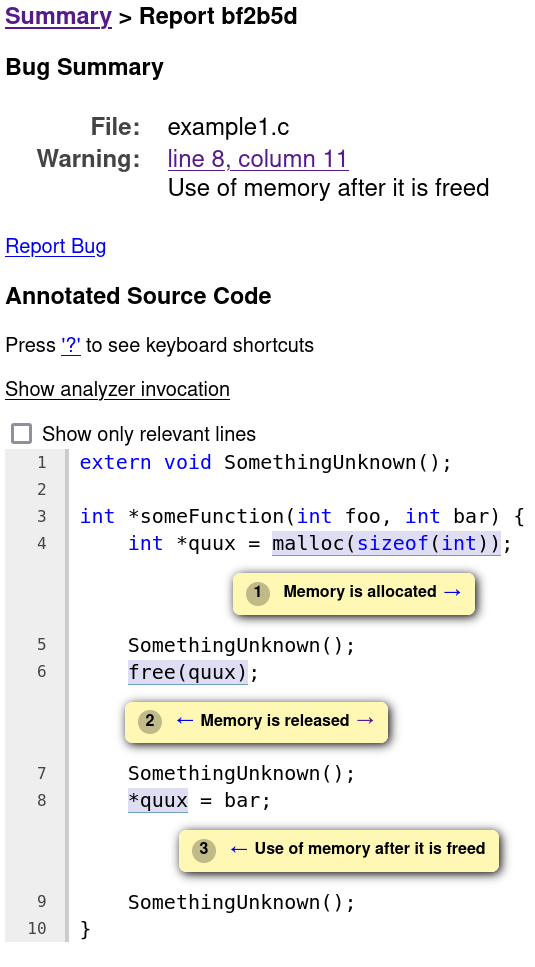
\includegraphics[height=0.9\textheight]{../static/scan-build-uaf-example1}
\end{frame}

\begin{frame}[fragile,label=useAfterFree2]{checking use-after-free (2)}
    \lstset{
        language=C,style=script,
        moredelim={**[is][\btHL<2>]{~2~}{~end~}},
    }
\begin{tikzpicture}
\node[anchor=north east] at (-.2, 0) {
\begin{lstlisting}
int *someFunction(int foo, int bar) {
    int *quux = malloc(sizeof(int));
    // A
    if (Complex(foo)) {
        free(quux);
        // B
    }
    ... /* omitted code that doesn't use quux */
    if (Complex(bar)) {
        // C
        *quux = bar;
    }
    ... /* omitted code that doesn't use quux */
    // D
}
\end{lstlisting}
};

    \tikzset{flow/.style={draw,thick,font=\fontsize{9}{10}\selectfont,anchor=north west},
    flowLine/.style={thick,-Latex}}
    \begin{scope}[y=0.8cm]
        \node[flow,dashed] (A) at (0, 0) { A: quux: \textit{allocated} };
        \begin{visibleenv}<2->
            \node[flow] (B) at (1, -1) { B: quux: \textit{freed} };
        \end{visibleenv}
        \begin{visibleenv}<3->
            \node[flow] (C1) at (1, -2) { C (from quux \textit{freed}): USE-AFTER-FREE };
        \end{visibleenv}
        \begin{visibleenv}<2->
            \node[flow] (D1) at (2, -3) { D (from quux \textit{freed})};
        \end{visibleenv}
        \begin{visibleenv}<4->
            \node[flow] (C2) at (1, -4) { C (from quux \textit{allocated}): ok };
            \node[flow] (D2) at (2, -5) { D (from allocated)};
        \end{visibleenv}
        \begin{visibleenv}<2->
            \draw[flowLine] ([xshift=.5cm]A.south west) |- ([yshift=.1cm]B.west);
        \end{visibleenv}
        \begin{visibleenv}<3->
            \draw[flowLine] ([yshift=-.1cm]B.west) -- ++(-.4cm, 0cm) |- ([yshift=.1cm]C1.west);
        \end{visibleenv}
        \begin{visibleenv}<2->
            \draw[flowLine] ([yshift=-.1cm]B.west) -- ++ (-.4cm,0cm) |- ([yshift=.1cm]D1.west);
        \end{visibleenv}
        \begin{visibleenv}<4->
            \draw[flowLine] ([xshift=.5cm]A.south west) |- ([yshift=.1cm]C2.west);
            \draw[flowLine] ([yshift=-.1cm]C2.west) -- ++(-.2cm,0cm) |- ([yshift=.1cm]D2.west);
            \draw[flowLine] ([xshift=.5cm]A.south west) |- ([yshift=.1cm]D2.west);
        \end{visibleenv}
    \end{scope}
    
    \begin{visibleenv}<4->
        \node[draw=red,very thick,fill=white,align=center,anchor=north west] at (-8, -6) {
            one idea: guess that Complex(foo) can be probably be true \\
            ~ \\
            option 1: say ``something wrong maybe''? \\
            option 2: try to figure out if Complex(foo) is true?)
        };
    \end{visibleenv}
\end{tikzpicture}
\end{frame}


\begin{frame}{result from clang's scan-build}
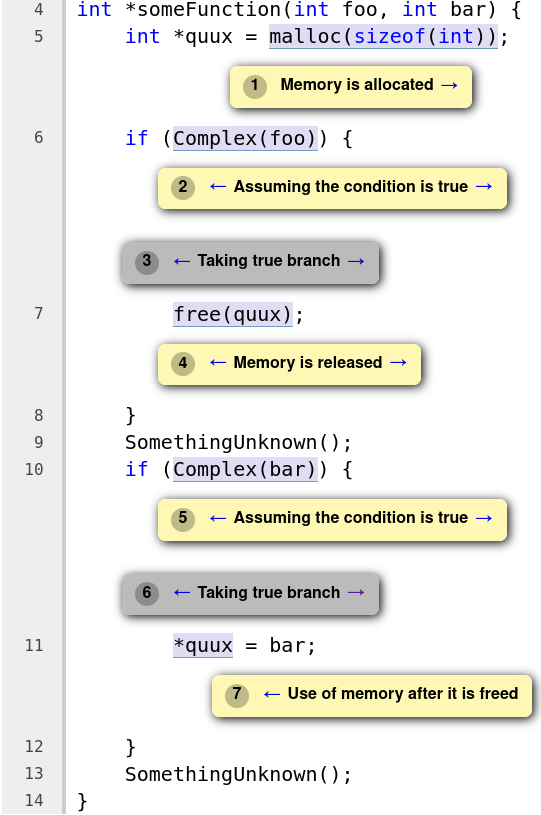
\includegraphics[height=0.9\textheight]{../static/scan-build-uaf-example2}
\end{frame}


    % FIXME: move loop discussion later

\subsection{exercise: aliasing and model}
\begin{frame}[fragile,label=homesModelExer]{exercise: holes in the model?}
\begin{tikzpicture}
\node (left) {
\begin{lstlisting}[language=C++,style=smaller]
void example(int a) {
    int *p;
    int *q;
    q = malloc(...);
    p = malloc(...);
    // (A)
    if (a > 0) {
        // (A1)
        p = q;
    }
    // (B)
    free(p);
    // (C)
    ...
}
\end{lstlisting}
};
\node[anchor=north west,align=left,draw,very thick] at (left.north east) {
exercise: what should state of pointer q be at C? \\
A. allocated \hspace{.5cm} B. freed \\
C. allocated if+only if reached via path with A1\\
D. freed if+only if reached via path with A1 \\
E. something else?
};
\end{tikzpicture}
\end{frame}

\begin{frame}{clang-analyzer output}
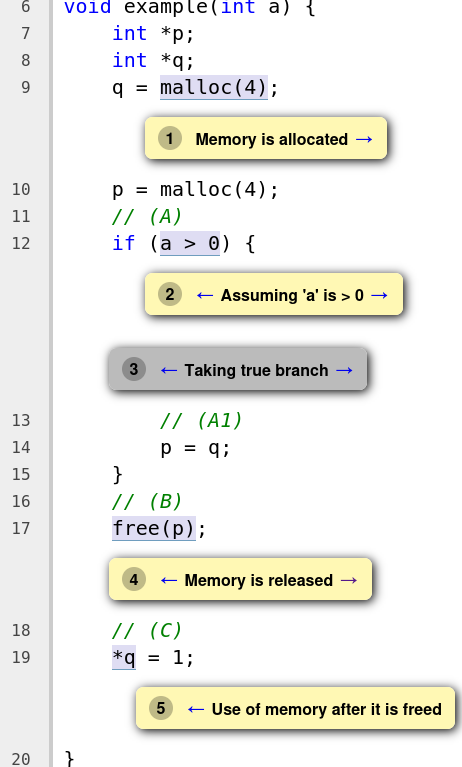
\includegraphics[height=0.9\textheight]{../static/clang-analyze-example4}
\end{frame}


\subsection{points-to analysis}
\usetikzlibrary{arrows.meta}

\begin{frame}{analysis building blocks}
    \begin{itemize}
    \item needed to track that \texttt{p} and \texttt{q} could point to same thing
    \vspace{.5cm}
    \item common prerequisite for all sorts of program analysis
    \end{itemize}
\end{frame}

\begin{frame}{overly simple algorithm for points-to analysis}
\begin{itemize}
\item for each pointer/reference track which objects it can refer to
\item if multiple paths: take union of all possible
\end{itemize}
\end{frame}

\begin{frame}[fragile,label=simplePointsTo]{simple points-to analysis}
\begin{lstlisting}[language=C++,style=smaller]
void example(int a) {
    int *p;
    int *q;
    q = malloc(...); // ID=1
    p = malloc(...); // ID=2
    // (A)
    if (a > 0) {
        p = q;
        // (B)
    }
    // (C)
    ...
}
\end{lstlisting}
\begin{tikzpicture}[overlay, remember picture]
    \tikzset{flow/.style={draw,thick,font=\fontsize{9}{10}\selectfont,anchor=north west,align=left},
    flowLine/.style={thick,-Latex}}
    \coordinate (base) at ([xshift=-9cm,yshift=-2cm]current page.north east);
    \begin{scope}[shift={(base)}]
        \begin{scope}
            \node[flow] (A) at (0, 0) { A: \myemph<2>{p (v1)}: \{ID=1\}; \myemph<2>{q (v1)}: \{ID=2\} };
            \node[flow] (B) at (1, -1) { B: \myemph<2>{p (v2)}: \{ID=2\}; \myemph<2>{q (v1)}: \{ID=2\} };
            \begin{visibleenv}<4->
            \node[flow] (C) at (0, -4) { C: \myemph<2>{p (v3)}: \myemph<3>{\{ID=1,ID=2\}}: \myemph<2>{q (v1)}: \{ID=2\} };
            \draw[flowLine] ([xshift=.5cm]A.south west) |- (B.west);
            \draw[flowLine] ([xshift=.5cm]B.south west) -- ([xshift=1.5cm]C.north west);
            \draw[flowLine] ([xshift=.5cm]A.south west) -- ([xshift=.5cm]C.north west);
            \end{visibleenv}
            \begin{visibleenv}<1-3>
            \node[flow] (C1) at (2, -2) { C via B: p (v2): \{ID=2\}: q (v1): \{ID=2\} };
            \node[flow] (C2) at (2, -3) { C not via B: p (v2): \{ID=1\}: q (v1): \{ID=2\} };
            \draw[flowLine] ([xshift=.5cm]A.south west) |- (B.west);
            \draw[flowLine] ([xshift=.5cm]B.south west) |- (C1.west);
            \draw[flowLine] ([xshift=.5cm]A.south west) |- (C2.west);
            \end{visibleenv}
        \end{scope}
        \begin{visibleenv}<2>
        \node[draw=red,very thick,align=left,font=\small] at (0, -6) {
            likely first step: mark different versions of p, q \\
            and track them as separate variables \\
            this way: can avoid storing set of values for q for every block of code \\
            (instead just point to q (v1) set)
        };
        \end{visibleenv}
        \begin{visibleenv}<4>
        \node[draw=red,very thick,align=left,font=\small] at (0, -6) {
            alternate idea: avoid path explosion by merging possible sets
        };
        \end{visibleenv}
        \begin{visibleenv}<3>
        \node[draw=red,very thick,align=left,font=\small] at (0, -6) {
            one idea: keep track of each path separately \\
            (but limit to how much one can do this)
        };
        \end{visibleenv}
    \end{scope}
\end{tikzpicture}
\end{frame}
 % FIXME: move earlier?

\subsection{complicating points-to analysis}
\begin{frame}{complicating points-to analysis}
    \begin{itemize}
    \item would like to analyze program function-at-a-time, but\ldots
        \begin{itemize}
        \item functions can change values shared by other functions
        \end{itemize}
    \item what about computed array indices?
    \item what about pointers to pointers?
    \item \ldots
    \vspace{.5cm}
    \item high false-positive solution:
        \begin{itemize}
        \item when incomplete info: assume value points to anything of right type
        \end{itemize}
    \item high false-negative solution:
        \begin{itemize}
        \item when incomplete info: assume value points to nothing
        \end{itemize}
    \end{itemize}
\end{frame}


\subsection{example: model for use-after-free, with loop}
\usetikzlibrary{arrows.meta}
\begin{frame}[fragile,label=useAfterFree3]{checking use-after-free (3)}
    \lstset{
        language=C,style=script,
        moredelim={**[is][\btHL<2>]{~2~}{~end~}},
    }
\begin{tikzpicture}
\node[anchor=north east] at (-.2, 0) {
\begin{lstlisting}
void someFunction() {
    int *quux = malloc(sizeof(int));
    ...
    // A
    do {
        // B
        ...
        if (anotherFunction()) {
            free(quux);
            // C
        }
        ...
        // D
    } while (complexFunction());
    ...
    // E
    *quux++;
    ...
}
\end{lstlisting}
};
    \tikzset{flow/.style={draw,thick,font=\fontsize{9}{10}\selectfont,anchor=north west},
    flowLine/.style={thick,-Latex},
    flowLineB/.style={very thick,dotted,-Latex},
    }
    \begin{scope}[y=0.8cm]
        \begin{visibleenv}<1->
        \node[flow] (A) at (0, 0) { A: \textit{allocated} };
        \node[flow,alt=<3>{red}{},alt=<1-2>{dashed}] (B) at (1, -1) { B (from \textit{allocated}): \textit{allocated} };
        \draw[flowLine] ([xshift=.5cm]A.south west) |- ([yshift=.1cm]B.west);
        \end{visibleenv}
        \begin{visibleenv}<2->
        \node[flow] (C1) at (1, -2) { C (from \textit{allocated}): quux: \textit{freed} };
            \node[flow,alt=<1-4>{dashed}{}] (D1) at (1, -3) { D (from \textit{freed}): \textit{freed} };
        \node[flow] (E1) at (2, -4) { E (from \textit{freed}): USE-AFTER-FREE };
        \draw[flowLine] ([yshift=-.1cm]B.west) -- ++(-.2cm, 0cm) |- ([yshift=.1cm]C1.west);
        \draw[flowLine] ([yshift=-.1cm]C1.west) -- ++(-.2cm, 0cm) |- ([yshift=.1cm]D1.west);
        \draw[flowLine] ([yshift=-.1cm]D1.west) -- ++(-.2cm, 0cm) |- ([yshift=.1cm]E1.west);
        \end{visibleenv}
        \begin{visibleenv}<3->
        \node[flow,alt=<3>{dashed}{}] (D2) at (1, -5) { D (from \textit{allocated}): \textit{allocated} };
        \draw[flowLine,alt=<3>{red}{}] ([yshift=-.1cm]B.west) -- ++(-.3cm, 0cm) |- ([yshift=.1cm]D2.west);
        \node[flow] (E2) at (2, -6) { E (from \textit{allocated}): ok };
        \draw[flowLine,alt=<3>{red}{}] ([yshift=-.1cm]D2.west) -- ++(-.2cm, 0cm) |- ([yshift=.1cm]E2.west);
        \end{visibleenv} 
        \begin{visibleenv}<4->
        \draw[flowLineB,alt=<4>{red}{}] ([yshift=-.1cm]D2.east) -- ++(2.5cm, 0cm) |- ([yshift=.1cm]B.east);
        \end{visibleenv} 
        \begin{visibleenv}<5->
            \node[flow,alt=<5>{dashed}{}] (B2) at (1, -7) { B (from \textit{freed}): \textit{freed} };
            \draw[flowLine,alt=<5>{red}{}] ([yshift=-.1cm]D1.west) -- ++(-.8cm, 0cm) |- ([yshift=.1cm]B2.west);
            \node[flow] (C2) at (1, -8) { C (from \textit{freed}): DOUBLE-FREE };
            \draw[flowLine] ([yshift=-.1cm]B2.west) -- ++(-.8cm, 0cm) |- ([yshift=.1cm]C2.west);
        \end{visibleenv} 
        \begin{visibleenv}<6->
            \draw[flowLineB,alt=<6>{red}{}] ([yshift=-.1cm]B2.east) -- ++(3cm, 0cm) |- ([yshift=.2cm]D1.east);
        \end{visibleenv}
    \end{scope}
\end{tikzpicture}
\end{frame}

\begin{frame}{result from clang's scan-build}
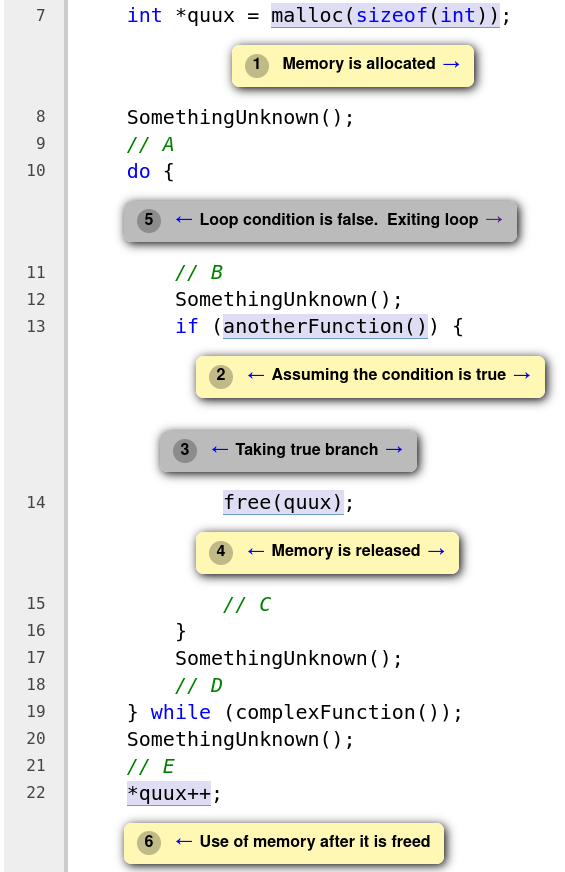
\includegraphics[height=0.9\textheight]{../static/scan-build-uaf-example3a}
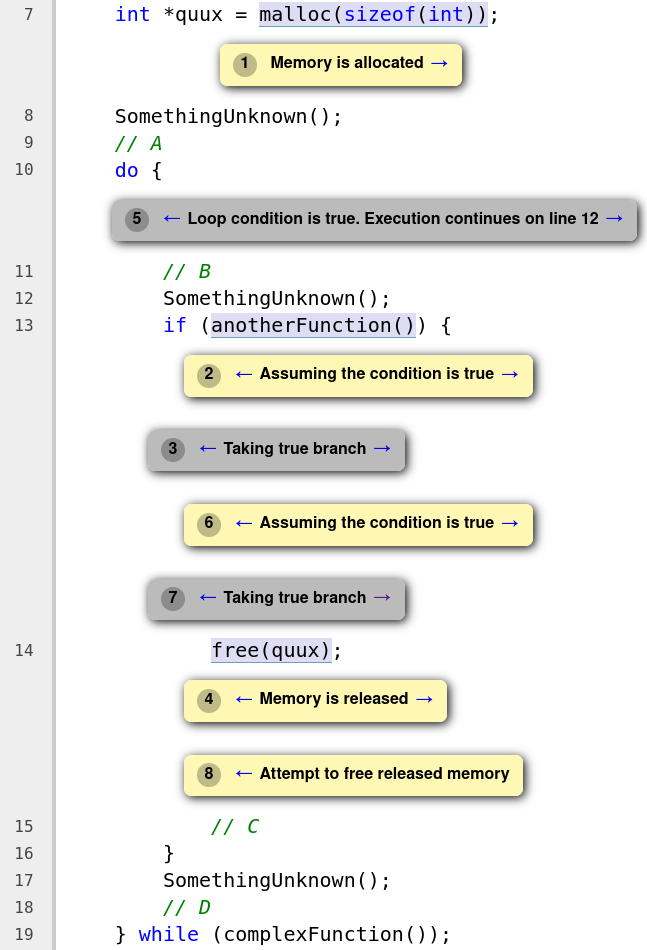
\includegraphics[height=0.9\textheight]{../static/scan-build-uaf-example3b}
\end{frame}


\subsection{example: model for array bounds}
\usetikzlibrary{arrows.meta}
\begin{frame}{checking for array bounds}
    \begin{itemize}
    \item can \textit{try} to apply same technique to array bounds
    \item but much more complicated/more likely to have false positives/negatives
    \vspace{.5cm}
    \item for each array or pointer track:  
        \begin{itemize}
        \item minimum number of elements before/after what it points to
        \end{itemize}
    \item for each integer track: 
        \begin{itemize}
        \item minimum bound
        \item maximum bound
        \end{itemize}
    \item similar analysis looking at paths?
    \end{itemize}
\end{frame}

\begin{frame}[fragile,label=bounds1]{checking array bounds (1)}
    \lstset{
        language=C,style=script,
        moredelim={**[is][\btHL<2>]{~2~}{~end~}},
    }
\begin{tikzpicture}
\node[anchor=north east] at (-.2, 0) {
\begin{lstlisting}
int array[100];
void someFunction(int foo) {
    // A
    if (foo > 100) {
        return;
    }
    // B
    array[foo] += 1;
}
\end{lstlisting}
};

    \tikzset{
        flow/.style={draw,thick,font=\fontsize{9}{10}\selectfont,anchor=north west},
        flowLine/.style={thick,-Latex},
    }
    \begin{scope}[y=1.2cm]
        \node[flow] (A) at (0, 0) { A: foo: $[-\inf, +\inf]$; array: indices [0, 99] };
        \node[flow] (B) at (0, -1) { B: foo: $[-\inf, +100]$; array: indices [0, 99] };
        \draw[flowLine] (A) -- (B);
    
    \begin{visibleenv}<2->
        \node[draw=red,very thick,fill=white,align=center] at (0, -4) {
            give warning about \texttt{foo == 100}? probably bug! \\
            give warning about \texttt{foo < 0}? maybe??
        };
    \end{visibleenv}
    \end{scope}
\end{tikzpicture}
\end{frame}

\begin{frame}[fragile,label=bounds2]{checking array bounds (2)}
    \lstset{
        language=C,style=script,
        moredelim={**[is][\btHL<2>]{~2~}{~end~}},
    }
\begin{tikzpicture}
\node[anchor=north east] at (-.2, 0) {
\begin{lstlisting}
int array[100];
void someFunction(int foo, bool bar) {
    int *p = array;
    // A
    p += 50;
    // B
    if (foo >= 50 || foo < 0) abort();
    // C
    if (bar) {
        foo = -foo;
    }
    // D
    p[foo] = 1;
}
\end{lstlisting}
};

    \tikzset{flow/.style={draw,thick,font=\fontsize{9}{10}\selectfont,anchor=north west},
    flowLine/.style={thick,-Latex}}
    \begin{scope}[y=1.2cm]
        \node[flow] (A) at (0, 0) { A: p: indices [0, 99]; foo: $[-\inf, +\inf]$ };
        \node[flow] (B) at (0, -1) { B: p: indices [-50, 49]; foo: $[-\inf, +\inf]$ };
        \node[flow] (C) at (0, -2) { C: p: indices [-50, 49]; foo: [0, 50] };
        \node[flow] (D1) at (-4, -3) { D (bar true): p: indices: [-50, 49]; foo: [-50, 0] } ;
        \node[flow,alt=<2>{draw=red}] (D2) at (1, -4) { D (bar false): p: indices: [-50, 49]; foo: [0, 50] };
        \draw[flowLine] (A) -- (B);
        \draw[flowLine] (B) -- (C);
        \draw[flowLine] (C) -- (D1);
        \draw[flowLine] (C) -- (D2);
    
    \begin{visibleenv}<2->
        \node[draw=red,very thick,fill=white,align=center] at (0, -6) {
            warn about possible out-of-bounds? 
        };
    \end{visibleenv}
    \end{scope}
\end{tikzpicture}
\end{frame}


\subsection{analysis for common insecure patterns}
\begin{frame}{common bug patterns}
    \begin{itemize}
    \item effectively detecting things like ``arrays are in bounds'' \\
        or ``values aren't used after being freed'' \\
        is not very reliable for large programs
    \item (but analysis tools are getting better)
    \vspace{.5cm}
    \item but static analysis tools shine for \myemph{common bug patterns}
    \end{itemize}
\end{frame}

\begin{frame}[fragile,label=suspectPatterns]{patterns clang's analyzer knows}
\begin{lstlisting}[language=C,style=smaller]
struct foo *p = malloc(sizeof(struct foo*)); // meant struct foo?
long *p = malloc(16 * sizeof(int)); // meant sizeof(long)?
\end{lstlisting}
\hrule
\begin{lstlisting}[language=C,style=smaller]
strncat(foo, bar, sizeof(foo));
\end{lstlisting}
\hrule
\begin{lstlisting}[language=C,style=smaller]
int *global;
int *foo() {
    int x;
    int *p = &x;
    ...
    global = p; // putting pointer to stack in global
    return p;    // returning pointer to stack
}
\end{lstlisting}
\end{frame}

\begin{frame}[fragile,label=suspectPatterns]{more suspect patterns }
    \begin{itemize}
    \item SpotBugs: Java static analysis tool
    \end{itemize}
\begin{lstlisting}[language=Java,style=smaller]
// pattern: connecting to database with empty password:
connection = DriverManager.getConnection(
    "jdbc:hsqldb:hsql://db.example.com/xdb" /* database ID */, 
    "sa" /* username */, "" /* password */);

// pattern: Sql.hasResult()'s second argument isn't a constant
Sql.hasResult(c, "SELECT 1 FROM myTable WHERE code='"+code+"'");

// pattern: new FileReader's argument comes from request
HttpRequest request = ...;
String path = request.getParameter("path");
BufferedReader r = new BufferedReader(
    new FileReader("data/" + path));
\end{lstlisting}
\end{frame}


\subsection{static analysis limits?}
\begin{frame}{static analysis}
    \begin{itemize}
    \item need to avoid exploring way too many paths
        \begin{itemize}
        \item clang-analyzer: only a procedure at a time
        \item other analyzers: some way of pruning paths
        \end{itemize}
    \item need to avoid false positives
        \begin{itemize}
        \item probably can't always assume every if can be true/false
        \item one idea: apply symbolic-execution like techniques to prune
        \item clang-analyzer: limited by being procedure-at-a-time
        \end{itemize}
    \end{itemize}
\end{frame}


\subsection{summary / actual tools}
\begin{frame}[fragile,label=practic]{static analysis practicality}
    \begin{itemize}
    \item good at finding some kinds of bugs
        \begin{itemize}
        \item array out-of-bounds probably not one --- complicated tracking needed
        \end{itemize}
    \item excellent for ``bug patterns'' like:
\begin{lstlisting}
struct Foo* foo;
...
foo = malloc(sizeof(struct Bar));
\end{lstlisting}
    \item false positive rates are often 20+\% or more
    \item some tools assume lots of annotations
    \item not limited to C-like languages
    \end{itemize}
\end{frame}

\begin{frame}{static analysis tools}
    \begin{itemize}
    \item Coverity, Fortify --- commerical static analysis tools
    \item Splint --- unmaintained?
        \begin{itemize}
            \item written by David Evans and his research group in the late 90s/early 00s
        \end{itemize}
    \item FindBugs (Java)
    \item clang-analyzer --- part of Clang compiler
    \item Microsoft's Static Driver Verifier  --- required for Windows drivers:
        \begin{itemize}
            \item mostly checks correct usage of Windows APIs
        \end{itemize}
    \end{itemize}
\end{frame}



\section{information flow}
\begin{frame}{information flow}
    \begin{itemize}
    \item so far: static analysis concerned with control flow
    \item often, we're really worried about how \textit{data} moves
    \vspace{.5cm}
    \item many applications:
        \begin{itemize}
        \item does an array index depend on user input?
        \item does an SQL query depend on user input?
        \item does data sent over network depend on phone number?
        \end{itemize}
    \item \ldots
    \vspace{.5cm}
    \item can do this \textit{statically} (potential dependencies) \\
         or \textit{dynamically} (actual dependencies as program runs)
    \end{itemize}
\end{frame}


\subsection{data flow graph}
\begin{frame}[fragile,label=infoFlowExample1a]{information flow graph (1a)}
\begin{lstlisting}[language=Python,style=smaller]
def f(a, b, c):
    desc = 'a={},b={}'.format(a, b)
    if b > 10:
        y = a
    else:
        y = c
    w = y + a
    pair = (w, c)
    desc = desc + \
         ',pair={}'.format(pair)
    print(desc)
    return y
\end{lstlisting}
\begin{tikzpicture}[overlay,remember picture]
\node[anchor=north east] at ([xshift=-.25cm,yshift=-1cm]current page.north east) {
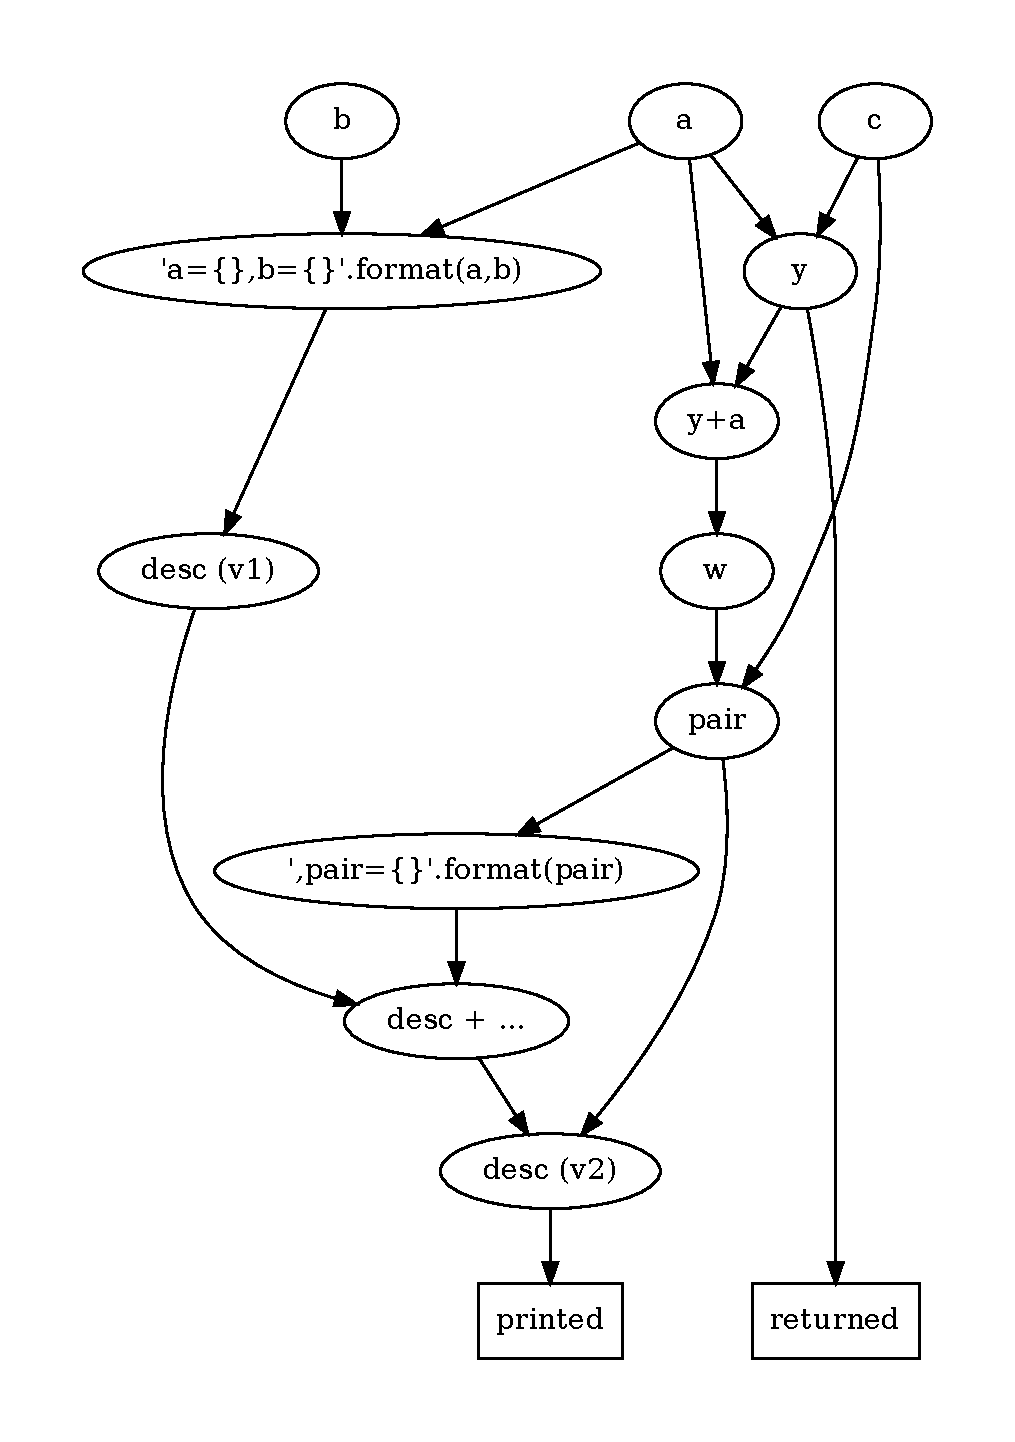
\includegraphics[width=0.4\textwidth]{../taint/info-flow-graph1}
};
\end{tikzpicture}
\end{frame}

\begin{frame}[fragile,label=infoFlowExample1b]{information flow graph (1b)}
\begin{itemize}
\item<2-> ex: does returned value depend on a, b, c?
\item<2-> ex: does value of pair depend on a, b, c?
\item<2-> ex: does printed value depend on a, b, c?
\end{itemize}
\begin{tikzpicture}[overlay,remember picture]
\node[anchor=north east] at ([xshift=-.25cm,yshift=-1cm]current page.north east) {
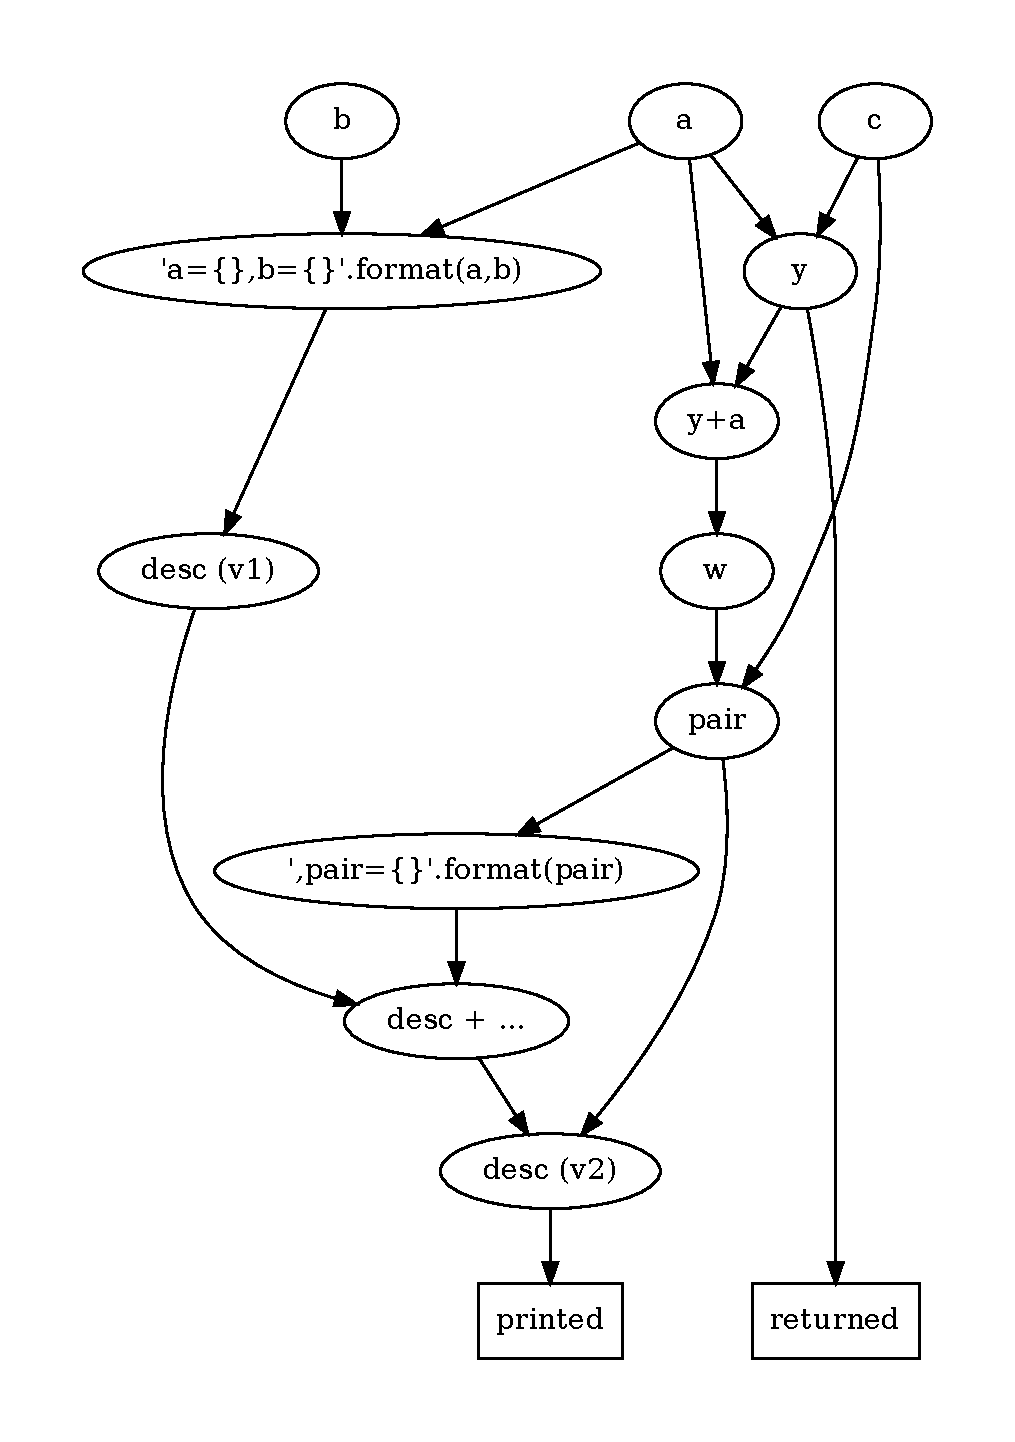
\includegraphics[width=0.4\textwidth]{../taint/info-flow-graph1}
};
\end{tikzpicture}
\end{frame}


\subsection{control flow versus information flow} 
\begin{frame}[fragile,label=infoFlowVControlFlow]{information flow and control flow}
\begin{lstlisting}[language=Python,style=smaller]
def f(a, b, c):
    if b > 10:
        y = a
    else:
        y = c
    return y
\end{lstlisting}
\begin{itemize}
\item Q: which is better \ldots
    \begin{itemize}
    \item if we're trying to see if user input makes it to SQL query?
    \item if we're trying to determine if private info goes out over network?
    \end{itemize}
\end{itemize}
\begin{tikzpicture}[overlay,remember picture]
\node[anchor=north east] (main) at ([xshift=-.25cm,yshift=-1cm]current page.north east) {
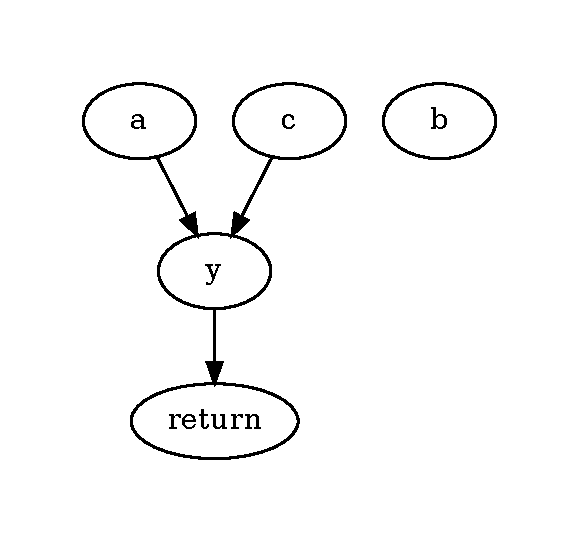
\includegraphics[width=0.3\textwidth]{../taint/info-flow-graph2}
};
\node[anchor=north east] (second) at (main.north west) {
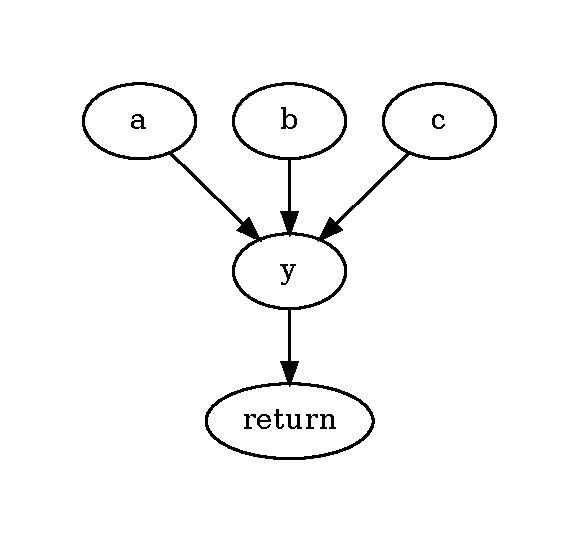
\includegraphics[width=0.3\textwidth]{../taint/info-flow-graph2b}
};
\end{tikzpicture}
\end{frame}


\subsection{challenges for data flow}
\begin{frame}[fragile,label=dFlowChallenges1]{static info flow challenges (1)}
\begin{tikzpicture}
\node (left) {
\begin{lstlisting}[language=Python,style=smaller]
# Python example
def stash(a):
    global y
    y = a
x = [0,1,2,3]
stash(x)
x[2] = input()
print(y[2])
\end{lstlisting}
};
\node[anchor=north west] at ([xshift=3cm]left.north east) {
\begin{lstlisting}[language=C++,style=smaller]
// C example
int *y;
void stash(int *a) {
    y = a;
}
int main() {
    int x[3];
    stash(x);
    y[2] = GetInput();
    printf("%d\n",x[2]);
}
\end{lstlisting}
};
\end{tikzpicture}
\begin{itemize}
\item same points-to problem with static analysis
\item need to realize that x[2] and y[2] are the same!
    \begin{itemize}
    \item even if assignment to/usage of y is more cleverly hidden
    \end{itemize}
\item can fix this with dynamic approach: monitor running program
\end{itemize}
\end{frame}

\begin{frame}[fragile,label=dFlowChallenges2]{static info flow challenges (2)}
\begin{tikzpicture}
\node (left) {
\begin{lstlisting}[language=Python,style=smaller]
def retrieve(flag):
    global the_default
    if flag:
        value = input()
    else:
        value = the_default
    value = process(value)
    if not flag:
        print("base on default: ",value)
    return value
retrieve(True)
retrieve(False)
\end{lstlisting}
};
\end{tikzpicture}
\begin{itemize}
\item input can't make it to print here
\item \ldots but need \textit{path-sensitive} analysis to tell
\item can fix this we dynamic approach: monitor running program
\end{itemize}
\end{frame}

\begin{frame}[fragile,label=dFlowChallenges3]{static info flow challenges (3)}
\begin{tikzpicture}
\node (left) {
\begin{lstlisting}[language=Python,style=smaller]
x = int(input())
if x == 0:
    print(0)
elif x == 1:
    print(1)
elif ...
\end{lstlisting}
};
\end{tikzpicture}
\begin{itemize}
\item does input make it to output?
\item should we try to detect this?
    \begin{itemize}
    \item probably depends on intended use of analysis
    \end{itemize}
\item harder to fix this issue
\end{itemize}
\end{frame}


\subsection{sources and sinks}
\begin{frame}{sources and sinks}
    \begin{itemize}
    \item needed choose \textit{sources} (so far: function arguments) \\
          and \textit{sinks} (so far: print, return)
    \item choice depends on application
    \item SQL injection: 
        \begin{itemize}
        \item sources: input from network
        \item sinks: SQL query functions
        \end{itemize}
    \item private info leak:
        \begin{itemize}
        \item sources: private data: phone number, message history, email, \ldots
        \item sinks: network output
        \end{itemize}
    \end{itemize}
\end{frame}


\section{taint tracking}

\begin{frame}{taint tracking idea}
    \begin{itemize}
        \item so far: looking at how information makes it from source to sink statically
        \item not actually running the program
        \vspace{.5cm}
        \item can do this as programs are running, trigger error
        \vspace{.5cm}
        \item \textit{dynamic taint tracking}
    \end{itemize}
\end{frame}




\subsection{implementations}

\begin{frame}{taint tracking implementations}
    \begin{itemize}
        \item for the programmer:
            \begin{itemize}
            \item supported as optional langauge feature --- Perl, Ruby
            \item doesn't seem to have gotten wide adoption?
            \end{itemize}
        \vspace{.5cm}
        \item for the malware analyst/user
            \begin{itemize}
            \item as part of a custom x86 VM (whole system, on machine code)
            \item as part of a custom Android system
            \item \ldots
            \end{itemize}
    \end{itemize}
\end{frame}


\subsection{taint tracking in perl}
\begin{frame}[fragile,label=perlTT1]{taint tracking in Perl (1)}
    \begin{minted}[fontsize=\small]{Perl}
#! perl -T
# -T: enable taint tracking
use warnings; use strict;
$ENV{PATH} = '/usr/bin:/bin';

print "Enter name: ";
my $name = readline(STDIN);
my $dir = $name . "-dir";

system("mkdir $dir");
\end{minted}
    \begin{itemize}
    \item ``Insecure dependency in system while running with -T switch at perltaint.pl line 10, <STDIN> line 1.''
    \end{itemize}
\end{frame}

\begin{frame}[fragile,label=perlTT2]{taint tracking in Perl (2)}
\begin{minted}[fontsize=\small]{Perl}
#! perl -T
# -T: enable taint tracking
use warnings; use strict;
$ENV{PATH} = '/usr/bin:/bin';

print "Enter name: ";
my $name = readline(STDIN);
# keep $name only if its all alphanumeric
# this marks $name as untainted
($name) = $name =~ /^([a-zA-Z0-9]+)$/;
my $dir = $name . "-dir";

system("mkdir $name");
\end{minted}
\end{frame}




\subsection{taint tracking asm}
\begin{frame}{taint tracking assembly}
\begin{itemize}
\item taint-tracking often proposed at \textit{assembly} level
\item examples:
\vspace{.5cm}
\item Panda.RE (2013--??)
    \begin{itemize}
    \item along with virtual machine record+replay
    \end{itemize}
\item Panaroma (Yin and Song, UC Berkeley, CCS '07)
\end{itemize}
\end{frame}

\begin{frame}{high-level overview}
\begin{itemize}
\item lookup table for each register and byte of memory:
    \begin{itemize}
    \item where did this value come from?
    \end{itemize}
\item \texttt{add \%r9, (\%r8)}: \\
    \texttt{memory-taint-table[register-values[R8]] =} \\
    \hspace{4cm} \texttt{register-taint-table[R9]}
\item also similar for virtual disk, network, \ldots
\item custom VM: all applications and the OS run with taint tracking
\end{itemize}
\end{frame}

\begin{frame}[fragile,label=panaromaSpecial]{Panaroma special cases}
\begin{itemize}
\item \texttt{xor \%eax, \%eax}: special case: remove taint from \%eax
\item Windows keyboard input did something like:
\begin{lstlisting}
keycode = GetFromKeyboard();
switch (keycode) {
case KEYCODE_A: return 'a';
case KEYCODE_B: return 'b';
...
}
\end{lstlisting}
\end{itemize}
\end{frame}

\begin{frame}{taint tracking for malware analysis}
\begin{itemize}
\item mark contents of file as tainted, then ID how used
    \begin{itemize}
    \item can find dependent conditional jumps/etc.
    \end{itemize}
\item figure out where network packet goes
    \begin{itemize}
    \item across processes with whole-virtual-machine analysis
    \end{itemize}
\vspace{.5cm}
\item can `tag' each byte of input differently
    \begin{itemize}
    \item identify which bytes of input jump depends on
    \end{itemize}
\end{itemize}
\end{frame}


\subsection{exercise: defeating} 
\begin{frame}[fragile,label=defeatAsmCheck]{defeating ASM-based checking}
\begin{itemize}
\item if a malware author wanted to defeat this taint checking,
what ideas seem promising for confusing the analysis?
\begin{itemize}
\item A. timing arithmetic operations to see if the machine is unusually slow
\item B. computing the hash of the malware's machine code and comparing it to a known value
\item C. changing \lstinline|x = y| to \\
    \lstinline|switch (x) { case 1: y = 1; break; case 2: ...}|
\item D. changing \lstinline|x = y| to \lstinline|x = z + y; x = x - z;|
\end{itemize}
\end{itemize}
\end{frame}


\subsection{obfuscation to defeat taint-tracking}
\begin{frame}{Tigress's transformation}
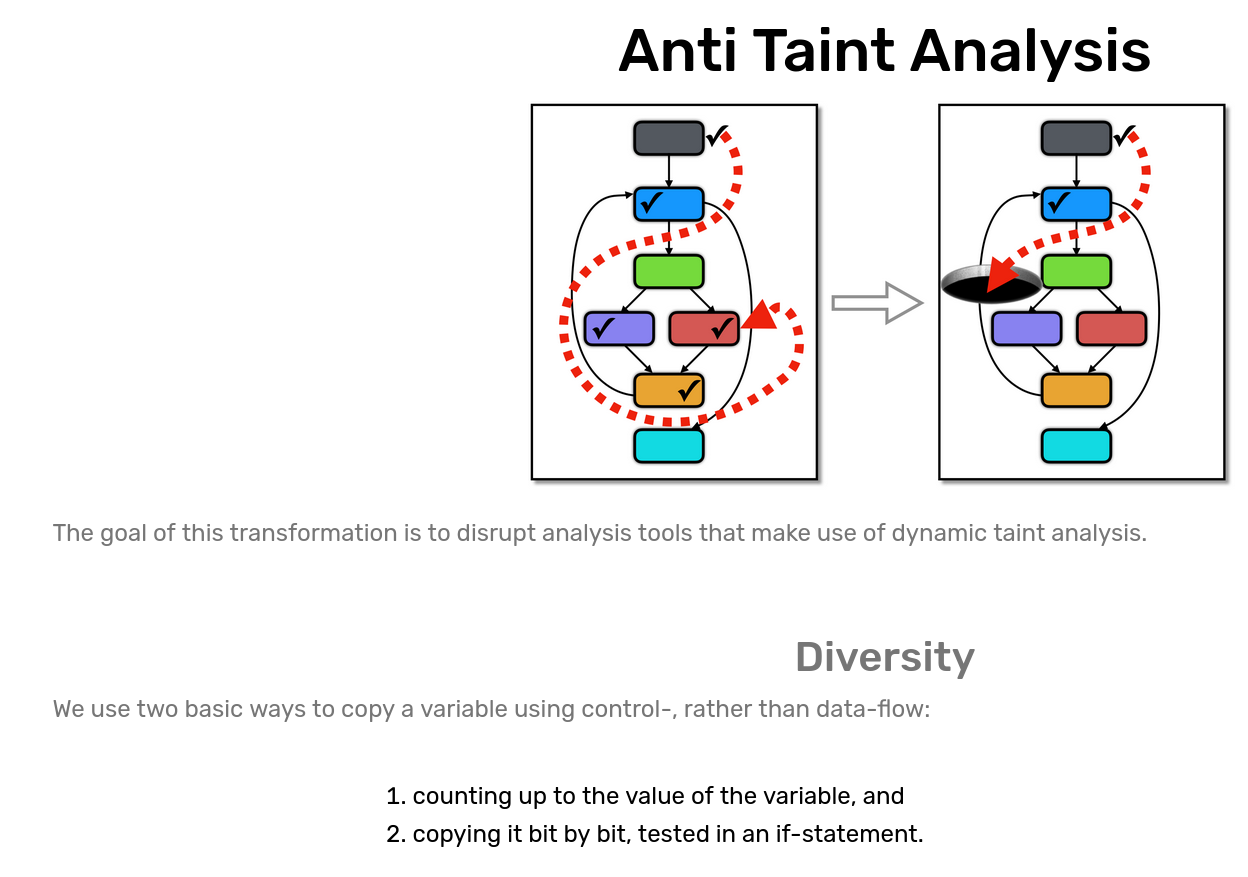
\includegraphics[height=0.9\textheight]{../taint/tigress-antitaint}
\end{frame}


\subsection{taint for finding mobile leaks}
\begin{frame}{example: TaintDroid}

\includegraphics[width=\textwidth]{../taint/taintdroid}
\end{frame}

\begin{frame}{TaintDroid instrumentation}
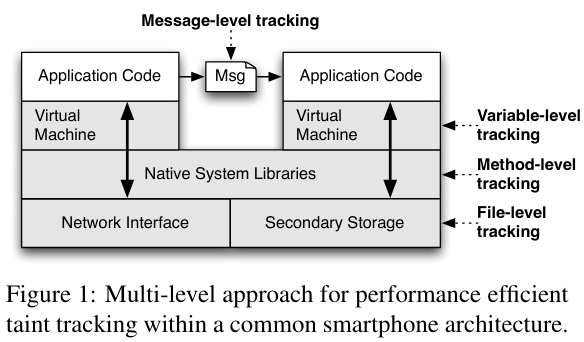
\includegraphics[height=0.9\textheight]{../taint/taintdroid-fig1}
\end{frame}

\begin{frame}{TaintDroid resutls}
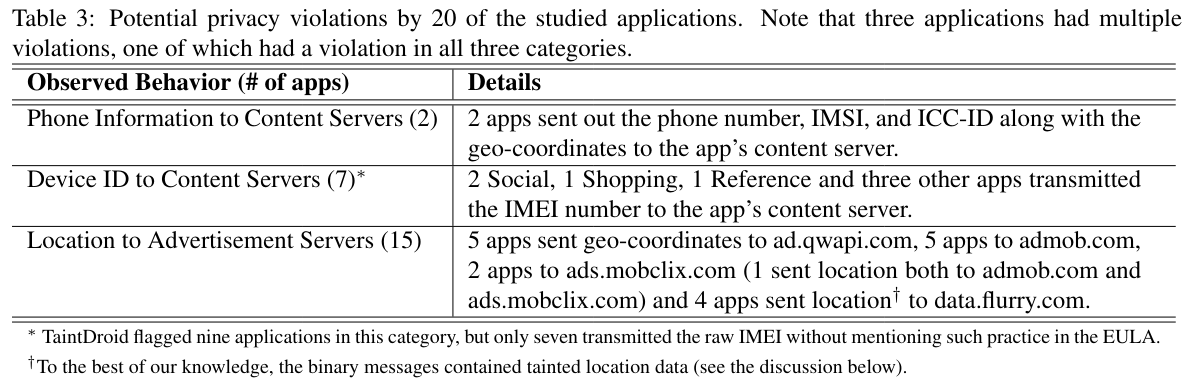
\includegraphics[width=\textwidth]{../taint/taintdroid-tbl3}
\end{frame}

\begin{frame}{TaintDroid and performance}
    \begin{itemize}
    \item modifying Dalvik ($\sim$ Java) VM allows good performance
    \item could do this sort of tracking on a ``live'' system
    \end{itemize}
\end{frame}


\section{Rust}

% FIXME

\subsection{general philosophy}

\begin{frame}{Rust philosophy}
    \begin{itemize}
    \item default rules that only allow `safe' things
        \begin{itemize}
        \item no dangling pointers
        \item no out-of-bounds accesses
        \end{itemize}
    \item escape hatch to use ``raw'' pointers or unchecked libraries
    \item escape hatch can be used to write useful libraries
        \begin{itemize}
            \item e.g. Vector/ArrayList equivalent
            \item \myemph{expose interface that is safe}
        \end{itemize}
    \end{itemize}
\end{frame}



\subsection{general syntax}
\usetikzlibrary{positioning,shapes.callouts}
\begin{frame}[fragile,label=rustHelloWorld1]{simple Rust syntax (1a)}
\begin{minted}{Rust}
fn main() {
    println!("Hello, World!\n");
}
\end{minted}
\end{frame}

\begin{frame}[fragile,label=rustHelloWorld1]{simple Rust syntax (1b)}
\begin{minted}{Rust}
fn main() {
    let name = "World";
    println!("Hello, {}!\n", name);
}
\end{minted}
\end{frame}

\begin{frame}[fragile,label=rustHelloWorld2]{simple Rust syntax (2)}
\begin{minted}[fontsize=\fontsize{11}{12}]{Rust}
fn timesTwo(number: i32) -> i32 {
    return number * 2;
}

/* or last value automatically returned: */
fn timesTwo(number: i32) -> i32 {
    number * 2
}
\end{minted}
\end{frame}

\begin{frame}[fragile,label=rustHelloWorld3]{simple Rust syntax (3)}
    \begin{minted}[fontsize=\fontsize{11}{12}]{Rust}
struct Student {
    name: String,
    id: i32,
}

fn get_example_student() -> Student {
    Student {
        name: String::from("Example Fakelastname"),
        id: 42,
    }
}
\end{minted}
\end{frame}

\begin{frame}[fragile,label=rustHelloWorld4]{simple Rust syntax (4)}
    \begin{minted}[fontsize=\fontsize{10}{11}\selectfont,escapeinside=||]{Rust}
fn factorial(number: i32) -> i32 {
    let mut|\tikzmark{mut}| result = 1;
    let mut index = 1;
    while index <= number {
        result *= index;
        index = index + 1;
    }
    return result;
}
\end{minted}
    \begin{tikzpicture}[overlay,remember picture]
        \coordinate (box) at (current page.center);
        \begin{visibleenv}<2>
            \node[my callout=mut,anchor=center,align=left] at ([yshift=2cm]box) {
                ``result'' is a mutable variable \\
                type automatically inferred as i32 (32-bit int)
            };
        \end{visibleenv}
    \end{tikzpicture}
\end{frame}



\subsection{references}
\subsubsection{basic example}
\begin{frame}[fragile,label=rustTimesTwoB]{Rust references}
\vspace{-.25cm}
    \begin{minted}[fontsize=\fontsize{10}{11}\selectfont,escapeinside=||]{Rust}
fn main() {
    let mut x: u32 = 42;

    {
        let y: &mut u32 = &mut x;
        *y = 100;
    }

    let z: &u32 = &x;

    println!("x = {}; z = {}", x, z);
}
\end{minted}
\end{frame}




\subsubsection{in context}

\usetikzlibrary{positioning,shapes.callouts}
\begin{frame}[fragile,label=rustTimesTwo]{Rust example with refs}
    \begin{minted}[fontsize=\fontsize{10}{11}\selectfont,escapeinside=||]{Rust}
use std::io;

fn main() {
    println!("Enter a number: ");

    let mut|\tikzmark{mut}| input = String::new();
    // could have also written:
    //   let mut input: String = String::new();
    
    io::stdin().read_line(&mut|\tikzmark{ref}| input);

    // parse number or fail with an error message
    let number: u32|\tikzmark{int}| = input.trim().parse()
        .expect("That was not a number!");
    println!("Twice that number is: {}", number * 2);
}
\end{minted}
    \begin{tikzpicture}[overlay,remember picture]
        \coordinate (box) at (current page.center);
        \begin{visibleenv}<2>
            \node[my callout=mut,anchor=center,align=left] at ([yshift=2cm]box) {
                ``input'' is a mutable variable \\
                type is automatically inferred as String
            };
        \end{visibleenv}
        \begin{visibleenv}<3>
            \node[my callout=ref,anchor=center,align=left] at ([yshift=-2cm]box) {
                pass mutable reference to input
            };
        \end{visibleenv}
        \begin{visibleenv}<4>
            \node[my callout=int,anchor=center,align=left] at (box) {
                number is an immutable unsigned 32-bit integer
            };
        \end{visibleenv}
    \end{tikzpicture}
\end{frame}




% FIXME: exercise: output with references

\subsection{basic ownership}
\begin{frame}{rules to stop dangling pointers (1)}
    \begin{itemize}
    \item objects have an single \myemph{owner}
    \item owner is the only one allowed to modify an object
    \item owner can give away ownership
    \item simplest version: only owner can access object
    \item never have multiple references to object --- always move/copy
    \end{itemize}
\end{frame}

\begin{frame}[fragile,label=rustOwnership1]{Rust objects and ownership (1a)}
    \begin{minted}[fontsize=\fontsize{9}{10}\selectfont]{Rust}
fn mysum(vector: Vec<u32>) -> u32 {
    let mut total: u32 = 0;
    for value in &vector {
        total += value
    }
    return total
}

fn foo() {
    let vector: Vec<u32> = vec![1, 2, 3];
    let sum = mysum(vector);
    // **moves** vector into mysum()
         // philosophy: no implicit expensive copies
    
    println!("Sum is {}", sum);
    // ERROR
    println!("vector[0] is {}" , vector[0]);
}
\end{minted}
    \begin{tikzpicture}[overlay,remember picture]
        \begin{visibleenv}<2>
            \node[anchor=center,font=\small,draw=black,ultra thick,fill=white] at (current page.center){
            \begin{lstlisting}[language={},style=script]
   Compiling lecture-demo v0.1.0 (file:///home/cr4bd/spring2017/cs4630/...
error[E0382]: use of moved value: `vector`
  --> src/main.rs:16:34
   |
13 |     let sum = mysum(vector);
   |                     ------ value moved here
...
16 |     println!("vector[0] is {}" , vector[0]);
   |                                  ^^^^^^ value used here after move
\end{lstlisting}
        };
        \end{visibleenv}
    \end{tikzpicture}
\end{frame}

\begin{frame}[fragile,label=rustOwnership2]{Rust objects and ownership (2)}
    \begin{minted}[fontsize=\fontsize{9}{10}\selectfont]{Rust}
fn mysum(vector: Vec<u32>) -> u32 {
    let mut total: u32 = 0
    for value in &vector {
        total += value
    }
    return total
}

fn foo() {
    let vector: Vec<u32> = vec![1, 2, 3];
    let sum = mysum(vector.clone());
    // give away a copy of vector instead
        // mysum will dispose, since it owns it
    
    println!("Sum is {}", sum);
    println!("vector[0] is {}" , newVector[0]);
}
\end{minted}
    \begin{tikzpicture}[overlay,remember picture]
        \begin{visibleenv}<2>
            \node[anchor=center,font=\small,draw=black,ultra thick,fill=white,align=center] at (current page.center){
            mysum borrows a copy
        };
        \end{visibleenv}
    \end{tikzpicture}
\end{frame}

\begin{frame}{moving?}
    \begin{itemize}
    \item moving a Vec --- really copying a pointer to an array and its size
    \item cloning a Vec --- making a copy of the array itself, too
    \vspace{.5cm}
    \item Rust defaults to moving non-trivial types
    \item some trivial types (u32, etc.) are copied by default
    \end{itemize}
\end{frame}

\begin{frame}[fragile,label=rustOwnership3]{Rust objects and ownership (3)}
    \begin{minted}[fontsize=\fontsize{9}{10}\selectfont]{Rust}
fn mysum(vector: Vec<u32>) -> (u32, Vec<u32>) {
    let mut total: u32 = 0
    for value in &vector {
        total += value
    }
    return (total, vector)
}

fn foo() {
    let vector: Vec<u32> = vec![1, 2, 3];
    let (sum, newVector) = mysum(vector);
    // give away vector, get it back
    
    println!("Sum is {}", sum);
    println!("vector[0] is {}" , newVector[0]);
}
\end{minted}
    \begin{tikzpicture}[overlay,remember picture]
        \begin{visibleenv}<2>
        \node[anchor=center,font=\small,draw=black,ultra thick,align=center,fill=white] 
            at (current page.center) {
        mysum ``borrows'' vector, then gives it back \\
        uses pointers
        };
        \end{visibleenv}
    \end{tikzpicture}
\end{frame}

\begin{frame}{ownership rules}
    \begin{itemize}
    \item exactly one owner at a time
    \item giving away ownership means you \myemph{can't use object}
        \begin{itemize}
        \item<2> common idiom --- temporarily give away object
        \end{itemize}
    \item either give object new owner or deallocate
    \end{itemize}
\end{frame}



\section{Rust: stopping dangling pointers}
\begin{frame}<1>[label=dangleRules]{rules to stop dangling pointers (2)}
    \begin{itemize}
    \item objects have an single \textbf{owner}
    \item owner can give away ownership permanently
        \begin{itemize}
        \item object is ``moved''
        \end{itemize}
    \item \myemph<1>{owner can let someone borrow object \myemph<2>{\textbf{temporarily}}}
        \begin{itemize}
        \item must know when object is given back
        \end{itemize}
    \item only \myemph<3>{\textbf{modify}} object when exactly one user
        \begin{itemize}
        \item owner or exclusive borrower
        \end{itemize}
    \end{itemize}
\end{frame}


% FIXME: exercise: which are compile errors?

\subsection{borrowing}

\begin{frame}[fragile,label=rustBorrowing1]{borrowing (1)}
    \begin{minted}[fontsize=\fontsize{10}{11}\selectfont]{Rust}
fn mysum(vector: &Vec<u32>) -> u32 {
    let mut total: u32 = 0
    for value in vector {
        total += value
    }
    return total
}

fn foo() {
    let vector: Vec<u32> = vec![1, 2, 3];
    let sum = mysum(&vector);
    // automates (vector, sum) = mysum(vector) idea
    
    println!("Sum is {}", sum);
    println!("vector[0] is {}" , vector[0]);
}
\end{minted}
\end{frame}

\begin{frame}[fragile,label=dangling1a]{dangling pointers? (1a)}
\begin{lstlisting}[language=C,style=small]
int *dangling_pointer() {
    int array[3] = {1,2,3};
    return &array[0]; // not an error
}
\end{lstlisting}
\hrulefill
    \begin{minted}[fontsize=\small]{Rust}
fn dangling_pointer() -> &mut i32 {
    let array = vec![1,2,3];
    return &mut array[0]; // ERROR
}
\end{minted}
\begin{tikzpicture}[overlay,remember picture]
    \begin{visibleenv}<2>
    \node[fill=white,draw,very thick,font=\scriptsize,align=left] at (current page.center) {
\begin{lstlisting}[language={},style=smaller]
error[E0106]: missing lifetime specifier
  --> src/main.rs:19:25
   |
19 | fn dangling_pointer() -> &mut i32 {
   |                          ^ expected lifetime parameter
   |
   = help: this function's return type contains a borrowed value,
           but there is no value for it to be borrowed from
\end{lstlisting}
};
    \end{visibleenv}
\end{tikzpicture}
\end{frame}

\begin{frame}[fragile,label=dangling1b]{dangling pointers? (1b)}
\begin{minted}[fontsize=\small]{Rust}
/* 'static = "valid forever" */
fn dangling_pointer() -> &'static mut i32 {
    let array = vec![1,2,3];
    return &mut array[0]; // ERROR
}
\end{minted}
\begin{tikzpicture}[overlay,remember picture]
    \begin{visibleenv}<2>
    \node[fill=white,draw,very thick,font=\scriptsize,align=left] at (current page.center) {
\begin{lstlisting}[language={},style=smaller]
error[E0515]: cannot return value referencing local variable `v`
 --> src/lib.rs:3:12
  |
3 |     return &v[0];
  |            ^-^^^
  |            ||
  |            |`v` is borrowed here
  |            returns a value referencing data owned
  |            by the current function
\end{lstlisting}
};
    \end{visibleenv}
\end{tikzpicture}
\end{frame}


\begin{frame}[fragile,label=dangling2]{dangling pointers? (2)}
\begin{lstlisting}[language=C,style=small]
int *ptr;
int dangling_pointer(int *array) {
    ptr = &array[0];
    return array[0];
}
\end{lstlisting}
\hrulefill
    \begin{minted}[fontsize=\small]{Rust}
static mut ptr : &i32 = &0;
fn dangling_pointer(v: Vec<i32>) -> i32 {
    ptr = &v[0];
    return v[0];
}
\end{minted}
\begin{tikzpicture}[overlay,remember picture]
    \begin{visibleenv}<3>
    \node[fill=white,draw,very thick,font=\scriptsize,align=left] at (current page.center) {
\begin{lstlisting}[language={},style=smaller]
error[E0133]: use of mutable static is unsafe
              and requires unsafe block
 --> src/lib.rs:3:5
  |
3 |     ptr = &v[0];
  |     ^^^ use of mutable static
  |
  = note: mutable statics can be mutated by
          multiple threads: aliasing violations
          or data races will cause undefined behavior
\end{lstlisting}
};
    \end{visibleenv}
    \begin{visibleenv}<2>
    \node[fill=white,draw,very thick,font=\scriptsize,align=left] at (current page.center) {
\begin{lstlisting}[language={},style=smaller]
error[E0597]: `v` does not live long enough
 --> src/lib.rs:3:12
  |
2 | fn dangling_pointer(v: Vec<i32>) -> i32 {
  |                     - binding `v` declared here
3 |     ptr = &v[0];
  |     -------^---
  |     |      |
  |     |      borrowed value does not live long enough
  |     assignment requires that `v` is borrowed for `'static`
4 |     return v[0];
5 | }
  | - `v` dropped here while still borrowed
\end{lstlisting}
};
    \end{visibleenv}
\end{tikzpicture}
\end{frame}

\begin{frame}[fragile,label=rustBorrowing2a]{borrowing (2a)}
\begin{minted}[fontsize=\fontsize{10}{11}\selectfont]{Rust}
fn add1(vector: &mut Vec<u32>) {
    for value in vector {
        *value += 1
    }
}

fn foo() {
    let mut vector: Vec<u32> = vec![1, 2, 3];
    add1(&mut vector);
    println!("vector[0] is {}" , vector[0]);
}
\end{minted}
\end{frame}

\begin{frame}[fragile,label=rustBorrowing2b]{borrowing (2b)}
\begin{minted}[fontsize=\fontsize{10}{11}\selectfont]{Rust}
fn add1(vector: &mut Vec<u32>) {
    for value in vector {
        *value += 1
    }
}

fn foo() {
    let mut vector: Vec<u32> = vec![1, 2, 3];
    // what previous example was basically shorthand for
    {
        let borrowed = &mut vector;
        // borrowing vector here...
        add1(borrowed);
        // until here
    }
    println!("vector[0] is {}" , vector[0]);
}
\end{minted}
\end{frame}


\begin{frame}{borrow tracking}
    \begin{itemize}
    \item compiler finds \textit{lifetime} of borrowing
        \begin{itemize}
        \item when is new reference to object created
        \item when is last use of reference to object
        \end{itemize}
    \item compiler checks for overlap with all other borrowings of that object
    \end{itemize}
\end{frame}



\subsection{lifetimes}
\againframe<2>{dangleRules}

\begin{frame}{lifetimes}
    \begin{itemize}
    \item every reference in Rust has a \myemph{lifetime}
    \item intuitively: how long reference is usable
    \item Rust compiler infers and checks lifetimes
    \end{itemize}
\end{frame}

\begin{frame}{lifetime rules}
    \begin{itemize}
    \item object is borrowed for duration of reference lifetime
        \begin{itemize}
        \item can't modify object during lifetime
        \item can't let object go out of scope during lifetime
        \end{itemize}
    \item lifetime of function args must include whole function call
    \item references returned from function must have lifetimes
        \begin{itemize}
        \item based on arguments or static (valid for entire program)
        \end{itemize}
    \item references stored in structs must have lifetime longer than struct
    \end{itemize}
\end{frame}

\begin{frame}[fragile,label=lifetimeHard]{lifetime inference}
\begin{minted}[fontsize=\small]{Rust}
fn get_first(values: &Vec<String>) -> &String {
    return &values[0];
}
\end{minted}
\begin{itemize}
    \item compiler infers lifetime of return value is same as input
\end{itemize}
\end{frame}

\begin{frame}[fragile,label=lifetimeHard2]{lifetime hard cases}
\begin{minted}[fontsize=\small]{Rust}
// ERROR:
fn get_first_matching(prefix: &str, values: &Vec<String>)
                            -> &String {
    for item in values {
        if item.starts_with(prefix) {
            return item
        }
    }
    panic!()
}
\end{minted}
\begin{itemize}
    \item this is a compile-error, because of the return value
    \item compiler need to be told lifetime of return value
\end{itemize}
\end{frame}

\begin{frame}[fragile,label=lifetimeAnnot]{lifetime annotations}
    \begin{minted}[fontsize=\fontsize{10}{11}\selectfont]{Rust}
fn get_first_matching<'a, 'b>(prefix: &'a str, values: &'b Vec<String>)
                            -> &'b String {
    for item in values {
        if item.starts_with(prefix) {
            return item
        }
    }
    panic!()
}
\end{minted}
\begin{itemize}
    \item prefix has lifetime $a$
    \item values and returned string have lifetime $b$
\end{itemize}
\end{frame}

\begin{frame}[fragile,label=lifetimeAnnot2]{lifetime annotations}
    \begin{minted}[fontsize=\fontsize{10}{11}]{Rust}
fn get_first_matching<'a, 'b>(prefix: &'a str, values: &'b Vec<String>)
                            -> &'b String {
    for item in values {
        if item.starts_with(prefix) {
            return item
        }
    }
    panic!()
}

fn get_first(values: &Vec<String>) -> &String {
    let prefix: String = compute_prefix();
    return get_first_matching(&prefix, values)
    // prefix deallocated here
}
\end{minted}
\end{frame}




\subsection{one writer}
\againframe<3>{dangleRules}

\begin{frame}[fragile,label=restrictMod]{restricting modification}
    \begin{minted}[fontsize=\fontsize{10}{11}\selectfont]{Rust}
fn modifyVector(vector: &mut Vec<u32>) { ... }
fn foo() {
    let vector: Vec<u32> = vec![1, 2, 3];
    for value in &vector {
        if value == 2 {
            modifyVector(&mut vector) // ERROR
        }
    }
}
    \end{minted}
\begin{itemize}
    \item trying to give away mutable reference
    \item \ldots while the for loop has a reference
    \vspace{.5cm}
    \item would be okay if giving away non-mutable reference
    \item why compiler distinguishes mutable/non-mutable references
\end{itemize}
\end{frame}




\subsection{concurrency}
\begin{frame}{data races}
    \begin{itemize}
    \item Rusts rules around modification built assuming concurrency
    \item OSes and other ``systems programming'' applications use multiple cores/threads
    \item particular problem: value being used from multiple threads at same time
    \end{itemize}
\end{frame}

\begin{frame}[fragile,label=raceUAF]{data races from use-after-free}
\begin{itemize}
\item given x: Rc<Foo> variable calling x.clone() on two cores
    \begin{itemize}
    \item some variable shared between two cores
    \item reference counting will prevent use-after-free, right?
    \end{itemize}
\end{itemize}
\begin{Verbatim}
x.clone on core A           x.clone on core B
-------------------------------------------
x.inc_strong():
  temp <- self.count
                            x.inc_strong():
                              temp <- self.count
                              self.count <- temp + 1
  self.count <- temp + 1
\end{Verbatim}
\begin{itemize}
\item problem: reference count one too low!
\end{itemize}
\end{frame}

\begin{frame}{Rust solution?}
\begin{itemize}
\item one option: require Rc implementation to handle mutiple cores
    \begin{itemize}
    \item problem: not zero overhead
    \end{itemize}
\item Rust solution: different types for multithreaded/multicore code
\item two ``traits'' to mark custom types:
    \begin{itemize}
    \item Sync: can be used from multiple cores/threads at once
    \item Send: can be moves from one thread to another
    \end{itemize}
\item two implementations of referenc counting
    \begin{itemize}
    \item Rc: not suitable for multicore, not marked Sync/Send
    \item Arc: is suitable for multicore, slower than Rc probably
    \end{itemize}
\end{itemize}
\end{frame}


\section{Rust: escape hatches and supporting dynamic allocation}
\begin{frame}{what about dynamic allocation?}
    \begin{itemize}
    \item saw Rust's Vec class --- equivalent to C++ vector/Java ArrayList
    \item idea: Vec wraps a heap allocation of an array
    \item owner of Vec ``owns'' heap allocation
        \begin{itemize}
        \item delete when no owner
        \end{itemize}
    \item also Box class --- wraps heap allocation of a single value
        \begin{itemize}
        \item basically same as Vec except one element
        \end{itemize}
    \end{itemize}
\end{frame}

    % FIXME: Rust 

\subsection{escape hatches implementing Vec}

\begin{frame}{escape hatch}
    \begin{itemize}
    \item Rust lets you avoid compiler's mechanisms
    \item implement your own
    \item \textbf{unsafe} keyword
    \item how Vec is implemented
    \end{itemize}
\end{frame}

\begin{frame}[fragile,label=insideVec]{deep inside Vec}
\begin{minted}[fontsize=\fontsize{9}{10}\selectfont]{Rust}
pub struct Vec<T> {
    buf: RawVec<T>, // interface to malloc
    len: usize,
}

impl<T> Vec<T> {
    ...
    pub fn truncate(&mut self, len: usize) {
        unsafe {
            // drop any extra elements
            while len < self.len {
                // decrement len before the drop_in_place(), so a panic on Drop
                // doesn't re-drop the just-failed value.
                self.len -= 1;
                let len = self.len;
                ptr::drop_in_place(self.get_unchecked_mut(len));
            }
        }
    }
    ...
}
\end{minted}
\end{frame}




\subsection{implementing new sharing schemes}
\begin{frame}<1>[fragile,label=escapeHatchSupportRc]{Rust escape hatch support}
    \begin{itemize}
        \item escape hatch: make new reference-like object
            \begin{itemize}
            \item (\ldots implemented by returning temporary `real' references)
            \end{itemize}
        \item<2> Rc: \verb|Rc<T>| acts like \verb|&T|
        \item callbacks on ownership ending (normally deallocation)
            \begin{itemize}
            \item Rust compiler enforces that ref-like object not in use when free call made
            \end{itemize}
        \item<2> Rc: deallocating \verb|Rc<T>| decrements shared count
        \item<2> Rc: real object only decremented on count == 0
        \item choice of what happens on copy
        \item<2> Rc: no implicit copy; explicit \verb|clone| operation increments count
    \end{itemize}
\end{frame}
 
\begin{frame}[fragile,label=refCounting]{alternative rule: reference counting}
    \begin{itemize}
    \item keep track of number of references
    \item increment count when making new `clone' of reference
    \item decrement when reference goes away
        \begin{itemize}
        \item Rust borrowing rules will enforce it is not used when this happens
        \end{itemize}
    \item delete when count goes to zero
        \begin{itemize}
        \item Rust automatically calls destructor --- no programmer effort
        \end{itemize}
    \item explicit operation to make new reference
    \item Rust implement with Rc type (``counted reference'')
    \end{itemize}
\end{frame}

\begin{frame}[fragile,label=refCountingEx]{Ref Counting Example}
\begin{minted}[fontsize=\fontsize{9}{10}\selectfont]{Rust}
struct Grade {
    score: i32, studentName: String, assignmentName: String,
}
struct Student {
    name: String,
    grades: Vec<Rc<Grade>>,
}
struct Assignment {
    name: String,
    grades: Vec<Rc<Grade>>
}

fn add_grade(student: &mut Student, assignment: &mut Assignment, score: i32) {
    let grade = Rc::new(Grade {
        score: score,
        studentName: student.name.clone(),
        assignmentName: assignment.name.clone(),
    })
    student.grades.push(Rc::clone(&grade));
    assignment.grades.push(Rc::clone(&grade));
    println!("Added grade with score={}", grade.score);
}
\end{minted}
\end{frame}

\againframe<2>{escapeHatchSupportRc}

\begin{frame}[fragile,label=rcImplA]{Rc implementation (approx) (0)}
\begin{minted}[fontsize=\fontsize{10}{11}\selectfont]{Rust}
struct RcInner<T: ?Sized> {
    strong: Cell<usize>,    // <-- count of Rc<T>s pointing to this
    weak: Cell<usize>,      // <-- count of Weak<T>s pointing to this
    value: T,               // <-- actual data
}

pub struct Rc<T: ?Sized> {
    ptr: NonNull<RcInner<T>>,
    phantom: PhantomData<RcInner<T>>, // <- so compiler infers what operations are safe better
}
\end{minted}
\begin{itemize}
\item NonNull = raw pointer wrapper
\item Cell = way to have mutable field of immutable object
\end{itemize}
\end{frame}



\begin{frame}[fragile,label=rcImplA]{Rc implementation (approx) (1)}
\begin{minted}[fontsize=\fontsize{10}{11}\selectfont]{Rust}
impl<T: ?Sized> Clone for Rc<T> {
    ... 
    fn clone(&self) -> Rc<T> {
        self.inc_strong(); // <-- increment reference count
        Rc { ptr: self.ptr }
    }
}
\end{minted}
\end{frame}

\begin{frame}[fragile,label=rcImplB]{Rc implementation (approx) (2)}
\begin{minted}[fontsize=\fontsize{10}{11}\selectfont]{Rust}
unsafe impl<#[may_dangle] T: ?Sized> Drop for Rc<T> {
    ...
    fn drop(&mut self) { // <-- compilers calls on deallocation
        unsafe {
            self.inner().dec_strong();
            if self.inner().strong() == 0 {
                self.drop_slow();
            }
        }
    }
    ...
}
\end{minted}
\end{frame}

\begin{frame}[fragile,label=rcImplC]{Rc implementation (approx) (3)}
\begin{minted}[fontsize=\fontsize{10}{11}\selectfont]{Rust}
impl<T: ?Sized> Deref for Rc<T> {
    type Target = T;

    #[inline(always)]
    fn deref(&self) -> &T {
        &self.inner().value
    }
}
\end{minted}
\begin{itemize}
\item observation: returned reference still has lifetime
\item compiler will enforce that extracted reference only used when Rc object valid
\end{itemize}
\end{frame}


\begin{frame}{Rc limitations}
    \begin{itemize}
    \item Rc: only gives references to \textit{read-only} objects
        \begin{itemize}
        \item cannot enforce ``only one mutable reference'' rule
        \end{itemize}
    \item Rc: allows memory leaks via circular references
        \begin{itemize}
        \item correct way to handle ciruclar references: Weak
        \item \ldots but not enforcement that it is used when needed
        \end{itemize}
    \end{itemize}
\end{frame}

\begin{frame}[fragile]{aside: Weak}
\begin{minted}[fontsize=\fontsize{10}{11}\selectfont]{Rust}
struct Foo {
    my_bar: Rc<Bar>,
    ...
}
struct Bar {
    my_foo: Weak<Foo>.
    ...
}
...
let bar: Bar = ...;
...
match bar.my_foo.upgrade() {
    Some(foo_rc) => {
        // foo_rc is an Rc<Foo>
        ...
    },
    None => {
        // the foo object was deleted
    }
}
\end{minted}
\end{frame}



\subsection{other Rust smart pointers}

\begin{frame}{other policies Rust supports}
    \begin{itemize}
        \item \myemph<2>{RefCell} --- borrowing, but check at runtime, not compile-time
            \begin{itemize}
            \item detect at runtime if used while already used
            \item internally: destructor call when returned object goes out of scope
            \end{itemize}
        \item Weak --- reference-counting, but don't contribute to count
            \begin{itemize}
            \item detect at runtime if used with count = 0
            \end{itemize}
        \item Mutex --- with multicore, enforce one user at a time by waiting
        \item \ldots
    \end{itemize}
\end{frame}




\section{zero-overhead}

\begin{frame}{zero-overhead}
    \begin{itemize}
    \item normal case --- lifetimes --- have no overhead
    \item compiler proves safety, generates code with no bookkeeping
        \vspace{.5cm}
    \item other policies (e.g. reference counting) do
    \item \ldots but can implement new ones if not good enough
    \end{itemize}
\end{frame}



\section{backup slides}
\begin{frame}{backup slides}
\end{frame}

\subsection{Rust linked list}
\begin{frame}[fragile,label=rLL]{Rust linked list}
    \begin{itemize}
    \item not actually a good idea
    \item use \verb|Box<...>| to represent object on the heap
    \item no null, use \verb|Option<Box<...>>| to represent pointer.
    \end{itemize}
\end{frame}

\begin{frame}[fragile,label=rustLL]{Rust linked list (not recommended)}
\begin{minted}[fontsize=\fontsize{9}{10}\selectfont]{Rust}
struct LinkedListNode {
    value: u32,
    next: Option<Box<LinkedListNode>>,
}

fn allocate_list() -> LinkedListNode {
    return LinkedListNode {
        value: 1,
        next: Some(Box::new(LinkedListNode {
            value: 2,
            next: Some(Box::new(LinkedListNode {
                value: 3,
                next: None
            }))
        }))
    }
}
\end{minted}
\end{frame}

\begin{frame}[fragile,label=rustLLNoBox1]{why the box? (1)}
\begin{minted}[fontsize=\fontsize{10}{11}\selectfont]{Rust}
struct LinkedListNode { // ERROR
    value: u32,
    next: Option<LinkedListNode>,
}

// error[E0072]: recursive type `LinkedListNode` has infinite size
\end{minted}
\end{frame}

\begin{frame}[fragile,label=rustLLNoBox2]{why the box? (2)}
\begin{minted}[fontsize=\fontsize{10}{11}\selectfont]{Rust}
struct LinkedListNode { // ERROR
    value: u32,
    next: Option<&LinkedListNode>,
}
// error[E0106]: missing lifetime specifier
//  --> src/main.rs:48:18
//    |
// 48 |     next: Option<&LinkedListNode>,
//    |                  ^ expected lifetime parameter
\end{minted}
\end{frame}



\subsection{other taint tracking uses}

\begin{frame}{taint tracking generally}
    \begin{itemize}
    \item taint tracking for other security issues is a big research area
    \item often by implementing taint tracking for assembly
        \begin{itemize}
        \item much, much higher overhead than implementing for Perl or Ruby
        \end{itemize}
            \only<2->{\hrulefill}
   \item<2->example: detect private information leaks
        \begin{itemize}
        \item taint personal information
        \item error if tainted info goes to network
        \end{itemize}
    \item<2-> example: check if \myemph{return addresses} are tainted before using
    \end{itemize}
\end{frame}


\end{document}
